\documentclass[11pt,a4paper]{report}

\usepackage[margin=2.4cm]{geometry}
\usepackage{amsmath,amssymb}
\usepackage{booktabs}
\usepackage{tikz}
\usepackage{pgfplots}
\pgfplotsset{compat=1.17}
\usetikzlibrary{arrows.meta,positioning,calc,shapes.geometric,fit,backgrounds,patterns}
\usepackage{xcolor}
\usepackage{tcolorbox}
\tcbuselibrary{skins,breakable}
\usepackage{fancyhdr}
\usepackage{titlesec}
\usepackage{enumitem}
\usepackage{caption}
\usepackage{longtable}
\usepackage[hidelinks]{hyperref}

\definecolor{acc}{HTML}{1F4E79}
\definecolor{warm}{HTML}{B7410E}
\definecolor{good}{HTML}{1B7A43}
\definecolor{lt}{HTML}{F2F6FA}
\definecolor{gr}{HTML}{666666}

\titleformat{\chapter}[display]
  {\normalfont\huge\bfseries\color{acc}}{\Large\chaptertitlename\ \thechapter}{8pt}{\Huge}
\titlespacing*{\chapter}{0pt}{-20pt}{20pt}

\pagestyle{fancy}
\fancyhf{}
\fancyhead[L]{\small\color{gr}FP2 on ReRAM --- A Complete Explanation}
\fancyhead[R]{\small\color{gr}\thepage}
\renewcommand{\headrulewidth}{0.4pt}

\newtcolorbox{keybox}[1]{colback=lt,colframe=acc,fonttitle=\bfseries,
  title={#1},breakable,left=6pt,right=6pt,top=5pt,bottom=5pt}
\newtcolorbox{warnbox}[1]{colback=warm!5,colframe=warm,fonttitle=\bfseries,
  title={#1},breakable,left=6pt,right=6pt,top=5pt,bottom=5pt}
\newtcolorbox{saybox}[1]{colback=good!5,colframe=good,fonttitle=\bfseries,
  title={#1},breakable,left=6pt,right=6pt,top=5pt,bottom=5pt}

\newcommand{\jargon}[1]{\textcolor{acc}{\textbf{#1}}}
% shorthand used from Ch.5 onward
\newcommand{\Rs}{R_{\mathrm{s}}}
\newcommand{\Gcol}{G_{\mathrm{col}}}

\begin{document}

%=====================================================================
\begin{titlepage}
\centering
\vspace*{2cm}
{\Huge\bfseries\color{acc} Block Size Is Tile Height\par}
\vspace{0.8cm}
{\LARGE Storing 2-Bit Floating-Point Neural Networks\\[4pt] Inside a ReRAM Crossbar\par}
\vspace{1.4cm}
{\Large\itshape A complete explanation, starting from\\ how a single memory cell works\par}
\vspace{2cm}

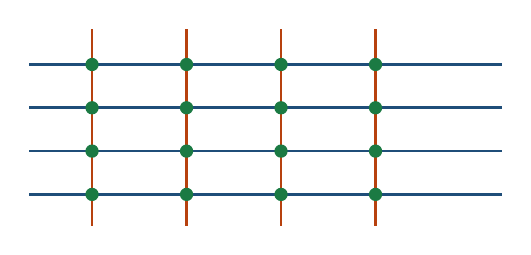
\begin{tikzpicture}[scale=1.0]
  % decorative crossbar
  \foreach \y in {0,0.55,1.1,1.65} {
    \draw[acc,line width=1pt] (0,\y) -- (6,\y);
  }
  \foreach \x in {0.8,2.0,3.2,4.4} {
    \draw[warm,line width=1pt] (\x,-0.4) -- (\x,2.1);
  }
  \foreach \y in {0,0.55,1.1,1.65} {
    \foreach \x in {0.8,2.0,3.2,4.4} {
      \fill[good] (\x,\y) circle (2.4pt);
    }
  }
\end{tikzpicture}

\vspace{2cm}
{\large Shaivi Nandi\par}
\vspace{0.3cm}
{\large International Institute of Information Technology, Bangalore\par}
\vspace{1.5cm}
{\large\today\par}
\end{titlepage}

%=====================================================================
\chapter*{How to read this document}
\addcontentsline{toc}{chapter}{How to read this document}

This document explains a research project from the ground up. It assumes you
know what a resistor is and what a neural network does, and nothing else.
Every piece of jargon is defined the first time it appears.

The story has one central idea, and if you remember only one thing, remember
this:

\begin{keybox}{The whole project in four sentences}
We store neural network weights as physical resistances in a memory chip, so
that multiplication happens through Ohm's law instead of in a digital
multiplier. When we did this the obvious way, the network's accuracy
collapsed from 92\% to 10\% --- no better than random guessing. We found the
cause was not random noise, as the published literature assumes, but a
\emph{predictable shrinking} of every output by a factor we can calculate in
advance. Dividing that factor back out recovers the accuracy exactly, and
because the shrinkage was the only thing limiting how large we could build the
array, removing it also made the design 13.6$\times$ more energy efficient.
\end{keybox}

\noindent\textbf{The structure:}

\begin{itemize}[leftmargin=1.4em]
  \item \textbf{Part I} explains the hardware: what a ReRAM cell is, how it
        stores a number, and how a grid of them multiplies.
  \item \textbf{Part II} explains the number format (FP2) and why it collides
        with the hardware. This collision is the problem the project solves.
  \item \textbf{Part III} derives the fix mathematically. This is the
        contribution.
  \item \textbf{Part IV} presents every experimental result, with the tables
        and the reasoning behind each.
  \item \textbf{Part V} is preparation for questions --- what is genuinely
        new, what was retracted and why, and what is not yet done.
\end{itemize}

\noindent Boxes are colour-coded: \textcolor{acc}{blue} for key ideas,
\textcolor{good}{green} for ``how to say this out loud'', and
\textcolor{warm}{orange} for warnings, limitations and honest caveats.

\tableofcontents

%=====================================================================
\part{The Hardware, From Scratch}
\chapter{What a ReRAM Cell Is}

\section{The one-sentence version}

A \jargon{ReRAM cell} (Resistive Random-Access Memory, also written RRAM) is a
sandwich of two metal electrodes with a thin insulating oxide between them.
Normally the oxide does not conduct. But if you apply a large enough voltage,
a microscopic conducting path forms through it, and the sandwich becomes a
conductor. Apply a large voltage the other way, and the path breaks.

\begin{figure}[h]
\centering
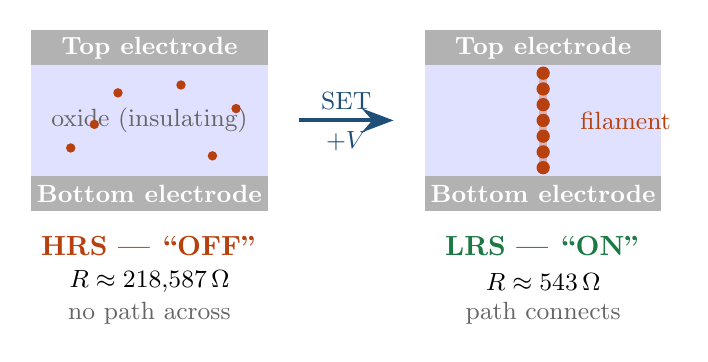
\begin{tikzpicture}[scale=1.0]
  % LEFT: HRS
  \begin{scope}[xshift=0cm]
    \fill[gray!60] (0,0) rectangle (3,0.45);
    \node[white,font=\small\bfseries] at (1.5,0.22) {Bottom electrode};
    \fill[blue!12] (0,0.45) rectangle (3,1.85);
    \node[font=\small,gr] at (1.5,1.15) {oxide (insulating)};
    \fill[gray!60] (0,1.85) rectangle (3,2.3);
    \node[white,font=\small\bfseries] at (1.5,2.07) {Top electrode};
    % scattered vacancies
    \foreach \p in {(0.5,0.8),(1.1,1.5),(2.3,0.7),(1.9,1.6),(2.6,1.3),(0.8,1.1)}
      \fill[warm] \p circle (1.7pt);
    \node[font=\bfseries,warm] at (1.5,-0.45) {HRS --- ``OFF''};
    \node[font=\small] at (1.5,-0.9) {$R \approx 218{,}587\,\Omega$};
    \node[font=\small,gr] at (1.5,-1.3) {no path across};
  \end{scope}
  % ARROW
  \draw[-{Stealth[length=4mm]},acc,line width=1.4pt] (3.4,1.15) -- (4.6,1.15)
     node[midway,above,font=\small,acc]{SET} node[midway,below,font=\small,acc]{$+V$};
  % RIGHT: LRS
  \begin{scope}[xshift=5cm]
    \fill[gray!60] (0,0) rectangle (3,0.45);
    \node[white,font=\small\bfseries] at (1.5,0.22) {Bottom electrode};
    \fill[blue!12] (0,0.45) rectangle (3,1.85);
    \fill[gray!60] (0,1.85) rectangle (3,2.3);
    \node[white,font=\small\bfseries] at (1.5,2.07) {Top electrode};
    % filament
    \foreach \y in {0.55,0.75,0.95,1.15,1.35,1.55,1.75}
      \fill[warm] (1.5,\y) circle (2.4pt);
    \draw[warm,line width=3pt,opacity=0.28] (1.5,0.5) -- (1.5,1.8);
    \node[font=\small,warm,anchor=west] at (1.85,1.15) {filament};
    \node[font=\bfseries,good] at (1.5,-0.45) {LRS --- ``ON''};
    \node[font=\small] at (1.5,-0.9) {$R \approx 543\,\Omega$};
    \node[font=\small,gr] at (1.5,-1.3) {path connects};
  \end{scope}
\end{tikzpicture}
\caption{A ReRAM cell in its two extreme states. Oxygen vacancies (orange)
scattered randomly leave the cell insulating (HRS). A voltage pulse lines them
up into a conducting \emph{filament}, and the cell becomes a good conductor
(LRS). The resistance values shown are the ones measured in our SPICE
calibration and used throughout this work.}
\end{figure}

\section{Why this is useful}

Three properties matter for us.

\textbf{It is non-volatile.} The filament stays where it is when power is
removed. A ReRAM cell remembers its value with no electricity at all. A
conventional SRAM cell needs six transistors constantly powered to hold one
bit; the moment you cut power, the bit is gone. This is why our standby power
comparison later shows $0$~mW against SRAM's $2.68$~mW --- not a small number,
but a structural zero.

\textbf{It is small.} One cell is essentially a via between two wires. An SRAM
bit needs six transistors laid out side by side. This is where the
$3.5\times$ density advantage in Chapter~10 comes from.

\textbf{It is analog.} This is the important one. The filament is not simply
present or absent --- you can grow it partially, by controlling how much
current you allow during the SET pulse. A partly-grown filament gives an
\emph{intermediate} resistance. So one cell can store more than one bit.

\begin{keybox}{Three states, not two}
We use three resistance states per cell:
\[
R_{\mathrm{LRS}} = 542.8\,\Omega, \qquad
R_{\mathrm{MID}} = 1099.8\,\Omega, \qquad
R_{\mathrm{HRS}} = 218{,}587\,\Omega
\]
The ratio $R_{\mathrm{HRS}}/R_{\mathrm{LRS}} = 403$ is called the
\jargon{on/off ratio}, and it is a headline figure of merit for a ReRAM
device. Ours is good; many published devices sit near 10.

Why stop at three? Because ReRAM reliability degrades sharply beyond three or
four levels --- the filament is a physical object of a few atoms, and asking
it to land reliably on eight distinguishable sizes is beyond what the device
does repeatably. Three is what the physics comfortably supports, and (as
Section~2.4 shows) three is exactly what our number format needs. That
coincidence is not luck; it is why the format was chosen.
\end{keybox}

\section{Conductance is the natural language}

Throughout this document we talk about \jargon{conductance} $G$ rather than
resistance $R$. They are reciprocals:
\[
G = \frac{1}{R}
\]
measured in siemens (S). The reason is Ohm's law. Written with resistance it
is a division, $I = V/R$; written with conductance it is a multiplication,
\[
\boxed{\,I = V \cdot G\,}
\]
and multiplication is what a neural network needs. This single line is the
entire reason analog in-memory computing exists.

\begin{table}[h]
\centering
\caption{Our three states in both languages.}
\begin{tabular}{lrrl}
\toprule
State & Resistance $R$ & Conductance $G$ & Meaning \\
\midrule
LRS  & $542.8\,\Omega$        & $1843\,\mu$S  & strong connection, ``big weight'' \\
MID  & $1099.8\,\Omega$       & $909\,\mu$S   & half connection, ``half weight'' \\
HRS  & $218{,}587\,\Omega$    & $4.6\,\mu$S   & almost nothing, ``zero weight'' \\
\bottomrule
\end{tabular}
\end{table}

Notice that HRS is not exactly zero conductance --- it is $4.6\,\mu$S, small
but real. That residual leakage matters later (Section~\ref{sec:levelerr}),
because it means our stored numbers do not land exactly on the values we
intended.

%=====================================================================
\chapter{How a Grid of Cells Multiplies}

\section{One cell is one multiplication}

Put a voltage $V$ across a cell of conductance $G$, and the current that flows
is $I = V\cdot G$. If we agree that the voltage represents an \emph{input
number} and the conductance represents a \emph{weight}, then the current is
their product. The chip did a multiplication, and it took no clock cycle, no
multiplier circuit, and essentially no energy. Physics did it.

\section{A column of cells is a dot product}

Now stack several cells so that their bottom ends all connect to the same
wire. Each cell $i$ has its own input voltage $V_i$ and its own conductance
$G_i$. Each contributes a current $V_i G_i$ into the shared wire, and
\jargon{Kirchhoff's current law} says currents joining at a node add up:
\[
I_{\mathrm{total}} = \sum_i V_i \, G_i
\]

That is a \jargon{dot product} --- multiply pairs, add the results. It is the
single operation that dominates every neural network. And here it happens in
one step, in the wire, for free.

\begin{figure}[h]
\centering
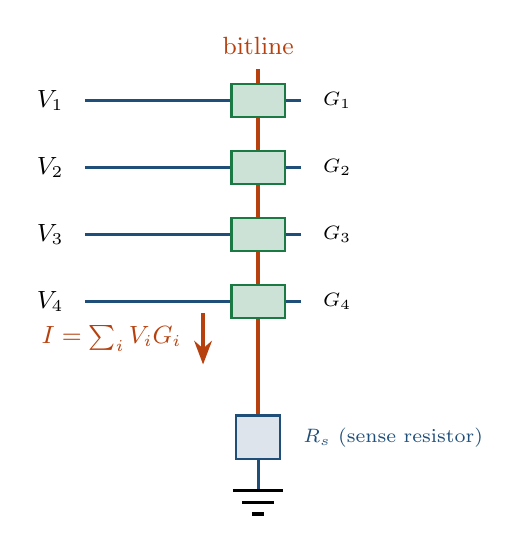
\begin{tikzpicture}[scale=1.0]
  % bitline first so opaque cells sit on top
  \draw[warm,line width=1.4pt] (2.0,3.4) -- (2.0,-1.0);
  \node[warm,font=\small] at (2.0,3.7) {bitline};
  \foreach \i/\v/\g in {0/{$V_1$}/{$G_1$},1/{$V_2$}/{$G_2$},2/{$V_3$}/{$G_3$},3/{$V_4$}/{$G_4$}} {
    \node[font=\small,anchor=east] at (-0.35,{3-\i*0.85}) {\v};
    \draw[acc,line width=1pt] (-0.2,{3-\i*0.85}) -- (2.55,{3-\i*0.85});
    \draw[fill=good!22,draw=good,line width=0.9pt]
       (2.0-0.34,{3-\i*0.85-0.21}) rectangle (2.0+0.34,{3-\i*0.85+0.21});
    \node[font=\scriptsize,anchor=west] at (2.7,{3-\i*0.85}) {\g};
  }
  % sense resistor to ground, laid out vertically to avoid collisions
  \draw[fill=acc!15,draw=acc,line width=0.9pt] (1.72,-1.0) rectangle (2.28,-1.55);
  \node[font=\scriptsize,acc,anchor=west] at (2.45,-1.28) {$R_s$ (sense resistor)};
  \draw[acc,line width=1.1pt] (2.0,-1.55) -- (2.0,-1.95);
  \draw[line width=1.2pt] (1.68,-1.95) -- (2.32,-1.95);
  \draw[line width=1.2pt] (1.80,-2.10) -- (2.20,-2.10);
  \draw[line width=1.2pt] (1.92,-2.25) -- (2.08,-2.25);
  % current annotation on the bitline, well clear of R_s
  \draw[-{Stealth[length=3mm]},warm,line width=1.2pt] (1.30,0.30) -- (1.30,-0.35);
  \node[font=\small,warm,anchor=east] at (1.15,-0.02) {$I=\sum_i V_i G_i$};
\end{tikzpicture}
\caption{A single crossbar column. Four inputs, four weights, one dot product,
computed by Kirchhoff's current law in the vertical wire. The current is read
by measuring the voltage across a small \emph{sense resistor} $R_s$ at the
bottom. That sense resistor is innocuous-looking and is the source of the
entire problem this project solves.}
\end{figure}

\section{A grid of cells is a matrix multiplication}

Add more columns. Every column sees the same input voltages but has its own
set of conductances, so every column computes a different dot product ---
against the same input vector. That is exactly a matrix--vector product:
\[
\mathbf{I} = \mathbf{G}^{\!\top}\mathbf{V}
\]

A grid of $M$ rows by $K$ columns performs $M\times K$ multiply-accumulate
operations in a single electrical settling time, which is nanoseconds. This
structure is called a \jargon{crossbar}, and a crossbar of a given size is
called a \jargon{tile}. The number of rows $M$ is the \jargon{tile height},
and it is the parameter this entire document is about.

\begin{keybox}{Why tile height is the parameter that matters}
At the bottom of every column sits an \jargon{ADC} (analog-to-digital
converter) that turns the analog current into a number the digital part of the
chip can use. ADCs are expensive --- in our design they consume roughly 55\%
of both the energy and the area of a tile.

You need one ADC per column regardless of how many rows the column has. So a
tile with 128 rows does four times as much work per ADC conversion as a tile
with 32 rows. \textbf{Taller tiles amortise the ADC cost over more
computation, and that is essentially the only lever available for improving
the energy efficiency of a crossbar accelerator.}

Everything that follows is a fight to make the tile taller.
\end{keybox}

\section{The problem of negative numbers}

Conductance cannot be negative. A resistor cannot push current backwards. But
neural network weights are negative about half the time, so we need a
representation for them.

The solution is \jargon{2T2R} --- two transistors, two resistors --- meaning
each weight gets \emph{two} cells on \emph{two} bitlines. One bitline
accumulates the positive parts, the other the negative parts, and we subtract
the two currents at the end:
\[
w_i \;\longrightarrow\; (G^p_i,\; G^n_i), \qquad
w_i \propto G^p_i - G^n_i
\]

\begin{figure}[h]
\centering
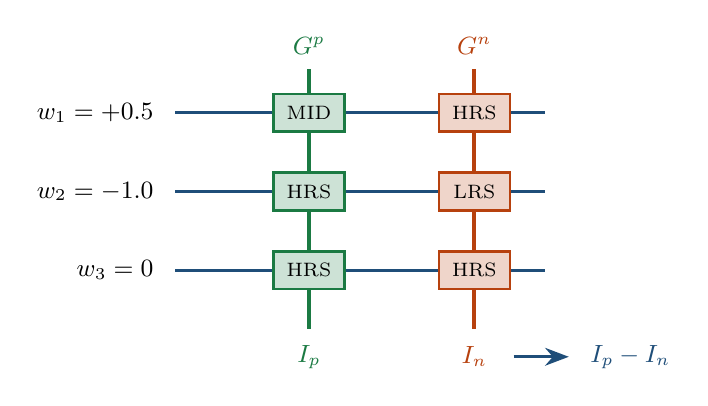
\begin{tikzpicture}[scale=1.0]
  % wordlines
  \foreach \i/\lbl in {0/{$w_1=+0.5$},1/{$w_2=-1.0$},2/{$w_3=0$}} {
    \node[font=\small,anchor=east] at (-0.35,{2.2-\i*1.0}) {\lbl};
    \draw[acc,line width=1pt] (-0.2,{2.2-\i*1.0}) -- (4.5,{2.2-\i*1.0});
  }
  % bitlines drawn FIRST so the opaque cell boxes sit on top of them
  \draw[good,line width=1.4pt] (1.5,2.75) -- (1.5,-0.55);
  \draw[warm,line width=1.4pt] (3.6,2.75) -- (3.6,-0.55);
  % cells: opaque boxes centred on each intersection
  \foreach \i/\st in {0/MID,1/HRS,2/HRS} {
    \draw[fill=good!22,draw=good,line width=0.9pt]
      (1.5-0.45,{2.2-\i*1.0-0.24}) rectangle (1.5+0.45,{2.2-\i*1.0+0.24});
    \node[font=\scriptsize] at (1.5,{2.2-\i*1.0}) {\st};
  }
  \foreach \i/\st in {0/HRS,1/LRS,2/HRS} {
    \draw[fill=warm!22,draw=warm,line width=0.9pt]
      (3.6-0.45,{2.2-\i*1.0-0.24}) rectangle (3.6+0.45,{2.2-\i*1.0+0.24});
    \node[font=\scriptsize] at (3.6,{2.2-\i*1.0}) {\st};
  }
  \node[good,font=\small] at (1.5,3.05) {$G^p$};
  \node[warm,font=\small] at (3.6,3.05) {$G^n$};
  \node[good,font=\small] at (1.5,-0.9) {$I_p$};
  \node[warm,font=\small] at (3.6,-0.9) {$I_n$};
  \draw[-{Stealth[length=3mm]},acc,line width=1.2pt] (4.1,-0.9) -- (4.8,-0.9);
  \node[acc,font=\small,anchor=west] at (4.95,-0.9) {$I_p - I_n$};
\end{tikzpicture}
\caption{2T2R differential encoding. A positive weight puts a low resistance
on the $+$ line and HRS on the $-$ line; a negative weight does the reverse; a
zero weight puts HRS on both. Subtracting the two column currents recovers a
signed result. Crucially for this project, \textbf{the two bitlines are read
separately}, which is what makes the fix in Chapter~6 possible.}
\end{figure}

\begin{table}[h]
\centering
\caption{Complete weight-to-cell mapping. Three resistance states are enough
to represent all five signed levels of our format.}
\begin{tabular}{crll}
\toprule
Weight level & $G^p$ cell & $G^n$ cell & Resulting current \\
\midrule
$+1.0$ & LRS & HRS & large positive \\
$+0.5$ & MID & HRS & small positive \\
$\phantom{+}0.0$ & HRS & HRS & $\approx 0$ \\
$-0.5$ & HRS & MID & small negative \\
$-1.0$ & HRS & LRS & large negative \\
\bottomrule
\end{tabular}
\end{table}

This is the coincidence promised earlier: five signed levels require only
three distinct \emph{magnitudes}, and three states is exactly what a ReRAM
cell holds reliably.

%=====================================================================
\part{The Number Format, and the Collision}
\chapter{FP2: Two Bits per Weight}

\section{Why weights need to be small}

A ResNet-18 network has about 11.16 million weights. Stored as standard
32-bit floats that is 44.6~MB, which does not fit on a chip. Every practical
accelerator therefore \jargon{quantizes} --- stores weights with fewer bits.

The extreme end of that spectrum is two bits per weight, a 16$\times$
reduction. The obvious way to spend two bits is four evenly spaced integers.
\jargon{FP2-E1M0} spends them differently.

\section{The format}

FP2-E1M0 means: 1 exponent bit, 0 mantissa bits, plus a sign. Each weight is
one of five levels:
\[
\{-1,\; -0.5,\; 0,\; +0.5,\; +1\}
\]

Two bits give four codes, and five levels need slightly more than that --- the
format packs a group of weights together to recover the difference. The
important point is not the bit-packing but the \emph{spacing}: the levels are
not evenly spaced. They cluster near zero.

\begin{figure}[h]
\centering
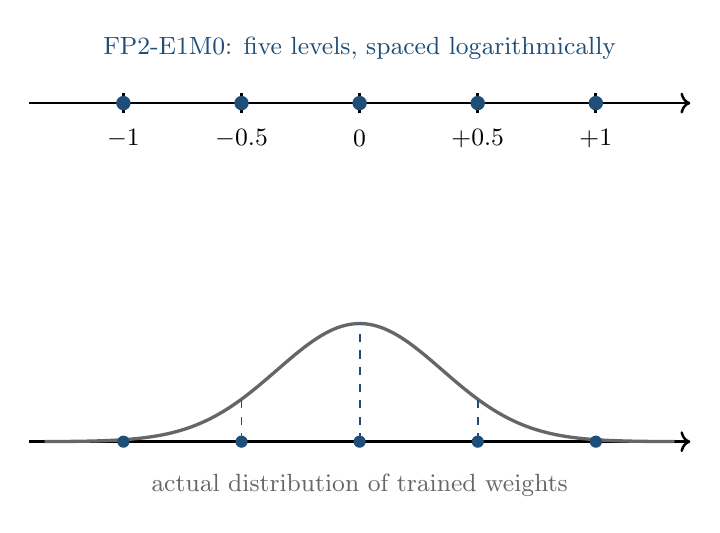
\begin{tikzpicture}[scale=1.0]
  \draw[->,line width=0.9pt] (-4.2,0) -- (4.2,0);
  \foreach \x/\l in {-3/{$-1$},-1.5/{$-0.5$},0/{$0$},1.5/{$+0.5$},3/{$+1$}} {
    \draw[line width=1pt] (\x,-0.13) -- (\x,0.13);
    \node[font=\small] at (\x,-0.45) {\l};
    \fill[acc] (\x,0) circle (2.6pt);
  }
  \node[font=\small,acc] at (0,0.7) {FP2-E1M0: five levels, spaced logarithmically};
  % bell curve
  \begin{scope}[yshift=-4.3cm]
    \draw[->,line width=0.9pt] (-4.2,0) -- (4.2,0);
    \draw[gr,line width=1.2pt,domain=-4:4,samples=90,smooth]
       plot (\x,{1.5*exp(-\x*\x/2.2)});
    \foreach \x in {-3,-1.5,0,1.5,3} {
      \draw[acc,dashed,line width=0.7pt] (\x,0) -- (\x,{1.5*exp(-\x*\x/2.2)});
      \fill[acc] (\x,0) circle (2.2pt);
    }
    \node[font=\small,gr] at (0,-0.55) {actual distribution of trained weights};
  \end{scope}
\end{tikzpicture}
\caption{Why unequal spacing wins. Trained neural-network weights are
bell-shaped --- most are near zero, few are large. Placing levels densely near
zero and sparsely at the extremes puts the precision where the weights
actually are. This is the same argument that makes floating point better than
fixed point.}
\end{figure}

\section{Block floating point: the shared scale}

Five fixed levels between $-1$ and $+1$ cannot represent a weight of $0.003$
or of $47$. The format solves this by \jargon{block floating point}: a group
of $B$ consecutive weights shares one 8-bit scale factor $s$, and the actual
weight is
\[
w_{\mathrm{actual}} = s \times \ell, \qquad \ell \in \{-1,-0.5,0,0.5,1\}
\]

Each block picks its own $s$ --- typically the largest magnitude in the block
--- so a block of tiny weights and a block of large weights both get full use
of the five levels.

\begin{keybox}{The block size $B$}
The FP2 specification fixes $B = 32$. Thirty-two consecutive weights share one
scale factor.

Storage cost: $32 \times 2$ bits for the levels, plus $8$ bits for the shared
scale, giving $2.25$ bits per weight. The scale is nearly free.

\textbf{Remember the number 32. The entire problem in Chapter~5 comes from
it.}
\end{keybox}

\section{Quantization-aware training}

Simply rounding a trained network's weights to five levels --- called
\jargon{post-training quantization} or PTQ --- loses accuracy, because the
network was never told this would happen.

\jargon{Quantization-aware training} (QAT) retrains the network with the
rounding simulated in the forward pass, so it learns weights that survive it.
The trick required is the \jargon{straight-through estimator}: rounding has
zero gradient everywhere, which would stop learning entirely, so during the
backward pass we pretend the rounding was the identity function and pass the
gradient through unchanged. Full-precision master weights are kept alongside
and are what actually get updated.

\begin{table}[h]
\centering
\caption{PTQ versus QAT on CIFAR-10, ResNet-18, full 10{,}000-image test set.}
\begin{tabular}{lrr}
\toprule
Configuration & Top-1 accuracy & Change vs FP32 \\
\midrule
FP32 baseline & 92.40\% & --- \\
FP2, post-training quantization & 87.88\% & $-4.52$ \\
FP2, 10 epochs of QAT & \textbf{92.44\%} & $\mathbf{+0.04}$ \\
\bottomrule
\end{tabular}
\end{table}

\begin{saybox}{How to say this}
``Two bits per weight sounds like it should be devastating. With
quantization-aware training it costs us nothing measurable on CIFAR-10 --- we
land four hundredths of a point \emph{above} the FP32 baseline, which is
within run-to-run noise. On the harder CIFAR-100 task it does cost about
1.25 points, and we report that rather than only quoting the favourable
result.''
\end{saybox}

%=====================================================================
\chapter{The Collision: Why Block Size \emph{Is} Tile Height}

\section{Two numbers that must be equal}

We now have two independent-looking parameters:

\begin{itemize}[leftmargin=1.4em]
  \item $B$, the block size of the number format --- how many weights share a
        scale factor. FP2 fixes this at 32.
  \item $M$, the tile height of the crossbar --- how many rows feed one
        column. The hardware wants this large, 128 or more, to amortise the
        ADC.
\end{itemize}

They look unrelated. They are not. \textbf{They are forced to be the same
number}, and understanding why is the key insight of the whole project.

\section{The argument}

A crossbar column physically produces \emph{one} current. That current is the
sum over every row in the column. To convert it back into a real number you
multiply by the block's shared scale factor $s$.

Now suppose a column spans two different blocks, with scales $s_1$ and $s_2$.
The current arriving at the ADC is
\[
I = \underbrace{\sum_{i \in \text{block 1}} V_i G_i}_{\text{needs }\times s_1}
  + \underbrace{\sum_{i \in \text{block 2}} V_i G_i}_{\text{needs }\times s_2}
\]
The two halves have already been added together by physics, in the wire,
before anything could be scaled. There is no way to apply two different
multipliers to one number after the fact. The information needed to separate
them is gone.

\begin{keybox}{$B = M$}
The block-floating-point block size and the crossbar tile height are not two
parameters. They are one physical parameter with two names.

FP2 says it must be 32. The crossbar says it should be 128 or more.
\textbf{They cannot both be satisfied.} That is the collision.
\end{keybox}

\begin{figure}[h]
\centering
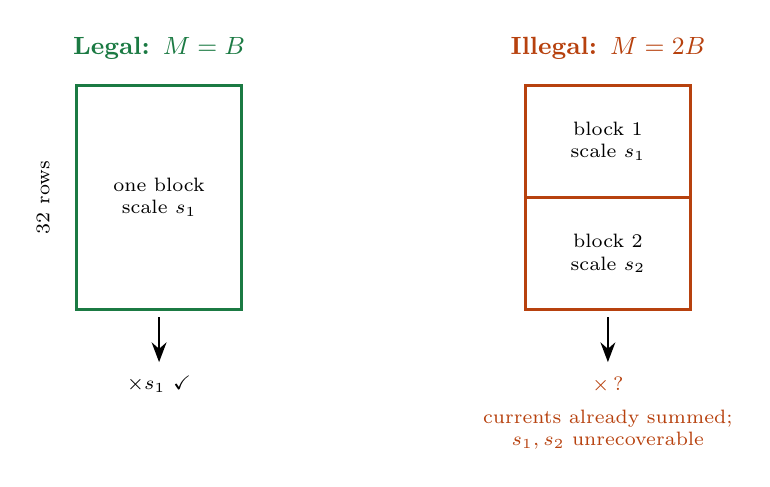
\begin{tikzpicture}[scale=0.95]
  % Left: aligned
  \begin{scope}
  \node[font=\bfseries\small,good] at (1.1,3.5) {Legal: $M = B$};
  \draw[good,line width=1.1pt] (0,0) rectangle (2.2,3);
  \node[font=\scriptsize,rotate=90] at (-0.45,1.5) {32 rows};
  \node[font=\scriptsize,align=center] at (1.1,1.5) {one block\\scale $s_1$};
  \draw[-{Stealth[length=2.5mm]},line width=1pt] (1.1,-0.1) -- (1.1,-0.7);
  \node[font=\scriptsize] at (1.1,-1.0) {$\times s_1$ \checkmark};
  \end{scope}
  % Right: spanning
  \begin{scope}[xshift=6cm]
  \node[font=\bfseries\small,warm] at (1.1,3.5) {Illegal: $M = 2B$};
  \draw[warm,line width=1.1pt] (0,1.5) rectangle (2.2,3);
  \draw[warm,line width=1.1pt] (0,0) rectangle (2.2,1.5);
  \node[font=\scriptsize,align=center] at (1.1,2.25) {block 1\\scale $s_1$};
  \node[font=\scriptsize,align=center] at (1.1,0.75) {block 2\\scale $s_2$};
  \draw[-{Stealth[length=2.5mm]},line width=1pt] (1.1,-0.1) -- (1.1,-0.7);
  \node[font=\scriptsize,warm] at (1.1,-1.0) {$\times\,?$};
  \node[font=\scriptsize,warm,align=center] at (1.1,-1.6)
     {currents already summed;\\$s_1,s_2$ unrecoverable};
  \end{scope}
\end{tikzpicture}
\caption{Why a tile cannot span two blocks. Once physics has added the
currents together, no downstream multiplier can undo the mixing.}
\end{figure}

\section{What happens if you build it anyway}

The natural response is: fine, ignore FP2's $B=32$ and just build a taller
tile with a matching larger block. We did exactly that, and measured the
accuracy of the real network running through the real circuit equations.

\begin{table}[h]
\centering
\caption{The collapse. CIFAR-10 Top-1, full 10{,}000-image test set.
``FP2 digital'' is the same quantized network evaluated in exact arithmetic;
``crossbar raw'' is the same network on the physical array.}
\begin{tabular}{crrr}
\toprule
$B = M$ & FP2 digital & Crossbar raw & Cost of the analog array \\
\midrule
32  & 92.42\% & 77.66\% & $-14.76$ \\
64  & 92.47\% & 57.54\% & $-34.93$ \\
128 & 92.81\% & 11.60\% & $-81.21$ \\
256 & 92.43\% & 10.00\% & $-82.43$ \\
\bottomrule
\end{tabular}
\end{table}

\begin{figure}[h]
\centering
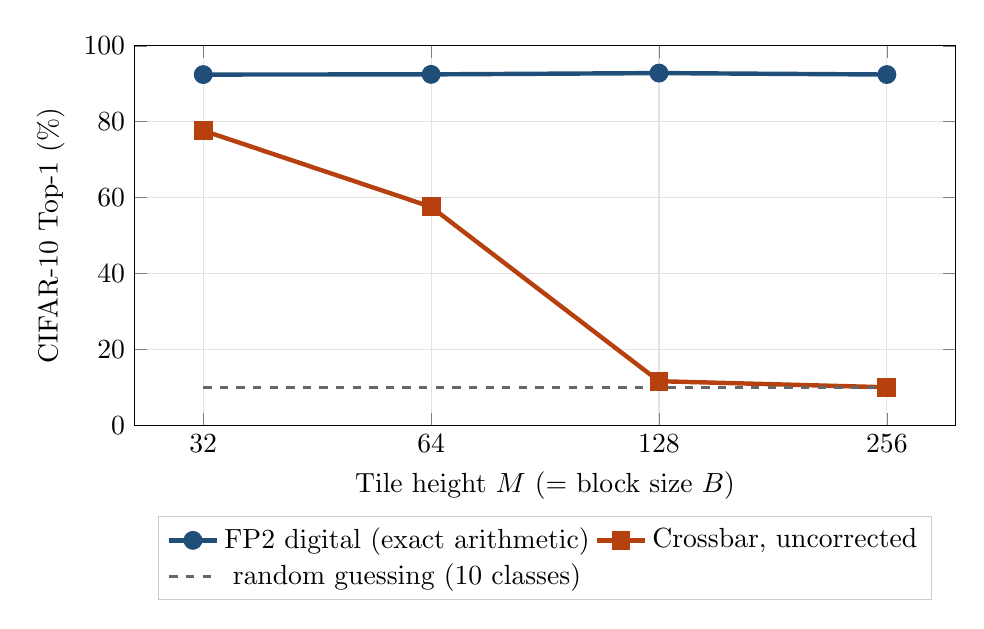
\begin{tikzpicture}
\begin{axis}[
  width=12cm,height=6.4cm,
  xlabel={Tile height $M$ (= block size $B$)},
  ylabel={CIFAR-10 Top-1 (\%)},
  xmode=log,log basis x=2,
  xtick={32,64,128,256},xticklabels={32,64,128,256},
  ymin=0,ymax=100,grid=major,grid style={gray!22},
  legend style={at={(0.5,-0.24)},anchor=north,legend columns=2,draw=gray!40},
]
\addplot[acc,line width=1.6pt,mark=*,mark size=2.6pt]
  coordinates {(32,92.42)(64,92.47)(128,92.81)(256,92.43)};
\addlegendentry{FP2 digital (exact arithmetic)}
\addplot[warm,line width=1.6pt,mark=square*,mark size=2.6pt]
  coordinates {(32,77.66)(64,57.54)(128,11.60)(256,10.00)};
\addlegendentry{Crossbar, uncorrected}
\addplot[gr,dashed,line width=1pt] coordinates {(32,10)(256,10)};
\addlegendentry{random guessing (10 classes)}
\end{axis}
\end{tikzpicture}
\caption{The central problem. Digital accuracy is flat --- the block size does
not bother the \emph{network} at all. But on the physical array, accuracy
falls off a cliff and reaches pure chance by $M=128$. At the tile height the
hardware wants, the chip has stopped computing anything.}
\end{figure}

\begin{saybox}{How to say this}
``At the block size FP2 specifies, the array already costs us fifteen accuracy
points. At the tile height that would actually make the hardware efficient,
the network outputs random guesses. So the format and the circuit are in
direct conflict, and this is the thing we set out to explain.''
\end{saybox}

%=====================================================================
\part{The Cause and the Fix}
\chapter{Diagnosing the Collapse}

\section{The suspect: the sense resistor}

Look again at the column diagram. The current leaving the column has to be
\emph{measured}, and the standard way is to pass it through a small known
resistor $R_s$ and measure the voltage that develops across it. Ours is
$20\,\Omega$ --- deliberately small, so as to disturb the circuit as little as
possible.

But $20\,\Omega$ is not zero. The moment current flows, the bottom of the
column lifts off ground by $I R_s$. And the voltage across each cell is the
difference between its input voltage and the bitline voltage. So lifting the
bitline \emph{reduces the voltage across every cell simultaneously}, which
reduces every cell's current, which is not what the ideal equation said.

\section{Deriving the error}

Let the column have cells $G_1 \dots G_M$ driven at voltages $V_1 \dots V_M$,
all feeding a bitline held at unknown voltage $v_b$, which drains to ground
through $R_s$. Kirchhoff's current law at the bitline node says everything
flowing in must flow out:
\[
\sum_i (V_i - v_b) G_i \;=\; \frac{v_b}{R_s}
\]
Expand and collect the $v_b$ terms:
\[
\sum_i V_i G_i \;=\; v_b\left(\frac{1}{R_s} + \sum_i G_i\right)
\]
which gives the bitline voltage in closed form:
\[
\boxed{\;v_b = \frac{\sum_i V_i G_i}{\dfrac{1}{R_s} + G_{\mathrm{col}}}\;},
\qquad G_{\mathrm{col}} \equiv \sum_i G_i
\]
The measured current is $I_{\text{actual}} = v_b / R_s$, and the ideal answer we
wanted was $I_{\text{ideal}} = \sum_i V_i G_i$. Dividing one by the other:
\[
\boxed{\;I_{\text{actual}} = \frac{I_{\text{ideal}}}{1 + R_s\,G_{\mathrm{col}}}\;}
\]

\begin{keybox}{Read that boxed equation carefully}
The output is the correct answer divided by $(1 + R_s G_{\mathrm{col}})$.

Now ask: what is in that denominator? Only $R_s$, which is a fixed component
value, and $G_{\mathrm{col}}$, the sum of the conductances programmed into that
column.

\textbf{The input voltages do not appear.} The error does not depend on the
data at all. It depends only on what we programmed into the array --- which we
chose, and therefore know exactly, at compile time.

This is not noise. It is a \emph{fixed, known, calculable gain}.
\end{keybox}

\section{Why the collapse gets worse with taller tiles}

$G_{\mathrm{col}}$ is a sum over $M$ cells. Double the tile height and you
roughly double it, which makes the denominator larger and the attenuation
worse. That is the exact shape of the collapse in Chapter~4.

\begin{table}[h]
\centering
\caption{Fraction of the ideal current that actually survives to the ADC.}
\begin{tabular}{lrrr}
\toprule
Tile height $M$ & 32 & 128 & 256 \\
\midrule
Current retained & 73.9\% & 41.5\% & 26.0\% \\
Signal lost & 26.1\% & 58.5\% & 74.0\% \\
\bottomrule
\end{tabular}
\end{table}

At $M=256$ three-quarters of the signal is gone before the ADC sees it. The
network is not confused --- it is being shouted at through a wall.

\section{Why the literature missed this}

\begin{warnbox}{A methodological point worth making in a viva}
The standard way to evaluate an analog CIM design is to model the analog error
as additive zero-mean Gaussian noise injected into the layer outputs. Nearly
every published simulator does this.

A zero-mean additive model \textbf{structurally cannot represent a systematic
gain}. It assumes the error averages to nothing over many terms. Our error is
a 26--74\% \emph{attenuation}, which never averages away.

An evaluation built on that assumption would have observed the accuracy
collapse, attributed it to noise accumulating in tall columns, concluded the
tile-height limit was fundamental, and stopped. We only saw the truth because
we solved the actual circuit equations. \textbf{Finding the fix required
throwing out the standard methodology}, and that is itself a contribution.
\end{warnbox}

%=====================================================================
\chapter{The Fix: Per-Column Gain Calibration}

\section{The idea}

If the output is the right answer multiplied by a known constant, multiply by
the reciprocal.

For column $j$, compute once, at compile time:
\[
c_j = 1 + R_s \sum_i G_{ij}
\]
and after reading the column, multiply the result by $c_j$.

That is the entire fix. One number per column. A multiplication that folds
into the block-scale multiply already present in the digital path, so it costs
no extra hardware at all.

\section{Doing it correctly with 2T2R}

There is a subtlety worth getting right, because the naive version does not
work.

The positive and negative bitlines have \emph{different} total conductances
--- they hold different cells --- so they suffer \emph{different} attenuation
factors. If you subtract first and correct afterwards, you are applying one
correction to a mixture of two differently-corrupted quantities, and it does
not cancel.

The order must be: read each bitline separately, correct each with its own
constant, \emph{then} subtract.

\begin{figure}[h]
\centering
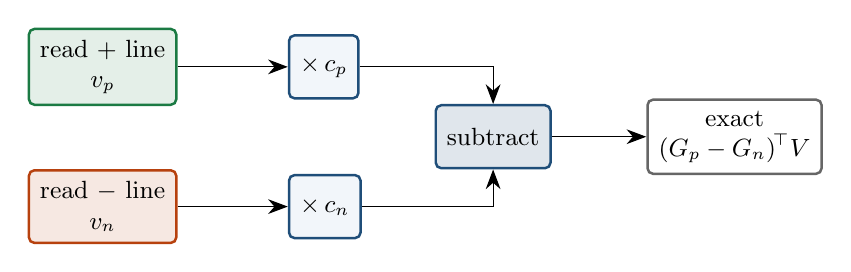
\begin{tikzpicture}[node distance=6mm,
   bx/.style={draw,line width=0.9pt,rounded corners=2pt,minimum height=8mm,
              font=\small,align=center,inner sep=4pt}]
  \node[bx,fill=good!12,draw=good] (a1) {read $+$ line\\$v_p$};
  \node[bx,fill=warm!12,draw=warm,below=8mm of a1] (a2) {read $-$ line\\$v_n$};
  \node[bx,fill=lt,draw=acc,right=14mm of a1] (b1) {$\times\,c_p$};
  \node[bx,fill=lt,draw=acc,right=14mm of a2] (b2) {$\times\,c_n$};
  \node[bx,fill=acc!14,draw=acc,right=14mm of $(b1)!0.5!(b2)$] (c) {subtract};
  \node[bx,fill=white,draw=gr,right=12mm of c] (d) {exact\\$(G_p-G_n)^{\!\top}V$};
  \draw[-{Stealth[length=2.5mm]}] (a1)--(b1);
  \draw[-{Stealth[length=2.5mm]}] (a2)--(b2);
  \draw[-{Stealth[length=2.5mm]}] (b1)-|(c);
  \draw[-{Stealth[length=2.5mm]}] (b2)-|(c);
  \draw[-{Stealth[length=2.5mm]}] (c)--(d);
\end{tikzpicture}
\caption{Correct order of operations. Each bitline is corrected by its own
constant \emph{before} the differential subtraction. Correcting after
subtracting does not cancel, because the two lines have different total
conductances.}
\end{figure}

\section{The algebra collapses}

Write it out. Each line, corrected:
\[
c_p \cdot \frac{(G_p^{\!\top}V)}{c_p} = G_p^{\!\top}V,
\qquad
c_n \cdot \frac{(G_n^{\!\top}V)}{c_n} = G_n^{\!\top}V
\]
and subtracting,
\[
\boxed{\;(G_p - G_n)^{\!\top} V\;}
\]
which is precisely the ideal matrix--vector product we wanted in the first
place. Not approximately. Exactly.

\section{It works}

\begin{table}[h]
\centering
\caption{The headline result. CIFAR-10 Top-1, full 10{,}000-image test set.}
\begin{tabular}{crrrr}
\toprule
$B = M$ & Crossbar raw & \textbf{Calibrated} & Recovered & FP2 digital ceiling \\
\midrule
32  & 77.66\% & \textbf{92.42\%} & $+14.76$ & 92.42\% \\
64  & 57.54\% & \textbf{92.47\%} & $+34.93$ & 92.47\% \\
128 & 11.60\% & \textbf{92.81\%} & $+81.21$ & 92.81\% \\
256 & 10.00\% & \textbf{92.43\%} & $+82.43$ & 92.43\% \\
\bottomrule
\end{tabular}
\end{table}

The calibrated column equals the digital ceiling at every tile height, to the
last digit. There is no residual error to trade off, because the correction is
algebraically exact rather than a fit.

\begin{figure}[h]
\centering
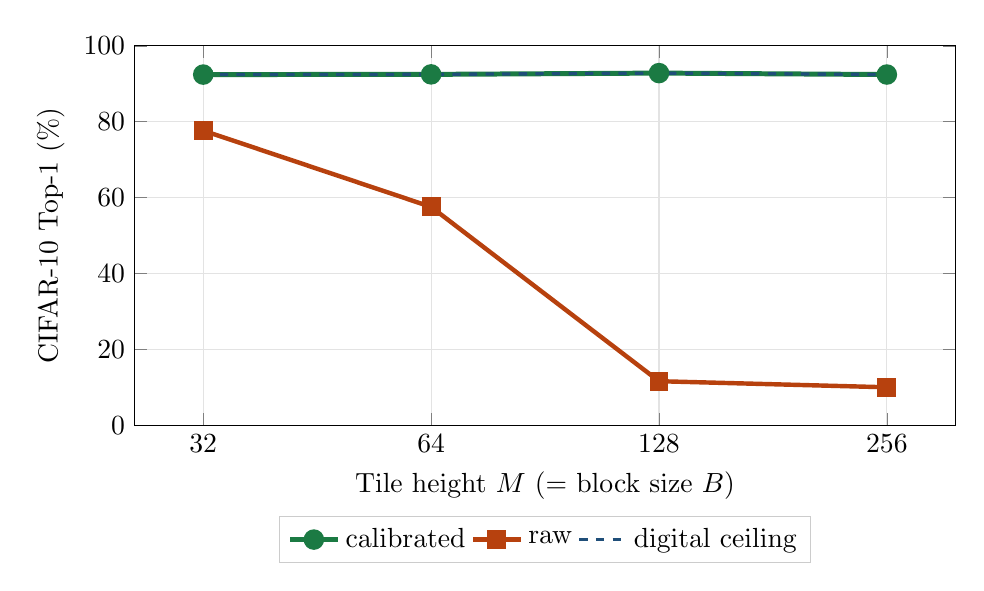
\begin{tikzpicture}
\begin{axis}[
  width=12cm,height=6.4cm,
  xlabel={Tile height $M$ (= block size $B$)},
  ylabel={CIFAR-10 Top-1 (\%)},
  xmode=log,log basis x=2,
  xtick={32,64,128,256},xticklabels={32,64,128,256},
  ymin=0,ymax=100,grid=major,grid style={gray!22},
  legend style={at={(0.5,-0.24)},anchor=north,legend columns=3,draw=gray!40},
]
\addplot[good,line width=1.8pt,mark=*,mark size=2.8pt]
  coordinates {(32,92.42)(64,92.47)(128,92.81)(256,92.43)};
\addlegendentry{calibrated}
\addplot[warm,line width=1.6pt,mark=square*,mark size=2.6pt]
  coordinates {(32,77.66)(64,57.54)(128,11.60)(256,10.00)};
\addlegendentry{raw}
\addplot[acc,dashed,line width=1.2pt]
  coordinates {(32,92.42)(64,92.47)(128,92.81)(256,92.43)};
\addlegendentry{digital ceiling}
\end{axis}
\end{tikzpicture}
\caption{The fix in one picture. The calibrated curve sits exactly on the
digital ceiling --- the dashed line is hidden underneath it --- while the
uncorrected curve falls to chance. Tile height has gone from a binding
constraint to a free design parameter.}
\end{figure}

\begin{saybox}{How to say this}
``The output is the correct answer divided by one plus $R_s$ times the column
conductance. That denominator contains no activation term --- it depends only
on the weights, which we programmed ourselves. So it is a constant we can
compute at compile time and simply divide back out. Because 2T2R already reads
both bitlines separately, correcting each one before the subtraction makes the
algebra collapse to the exact ideal product. One constant per column, folded
into a multiply that already exists in the datapath, and the accuracy comes
back completely.''
\end{saybox}

\section{An unexpected consequence: the sense resistor becomes free}
\label{sec:rsensefree}

There is a second payoff, and it took an outside paper to notice it.

Roy, Patil and Shanbhag (ISCAS 2022) worked out analytically what limits the
accuracy of any resistive crossbar. They found that the sensing resistance has
an \emph{optimum}. Too small and the signal is weak, so the ADC's quantisation
steps eat it. Too large and the signal clips against the converter's range.
The two effects balance at one value, and for ReRAM they put that value at
$835\,\Omega$.

Our design used $20\,\Omega$ --- forty times smaller. Not by analysis, but by
necessity: the loading error $1+R_s G_{\mathrm{col}}$ grows with $R_s$, so an
uncalibrated array is pushed toward the smallest sense resistor it can
tolerate, and pays for that with a weak signal.

Calibration removes the loading term exactly. So the reason for staying small
disappears. That is a testable prediction, and it was tested.

\begin{table}[h]
\centering
\caption{Sensing resistance sweep, $B{=}M{=}128$, 6-bit ADC, full 10\,000-image
test set. Digital ceiling $92.81\%$.}
\begin{tabular}{rrrr}
\toprule
$R_s$ ($\Omega$) & Raw & Calibrated & Gap \\
\midrule
20   & 11.61\% & 92.43\% & $-0.38$ \\
100  & 10.00\% & 92.62\% & $-0.19$ \\
200  & 10.00\% & 92.59\% & $-0.22$ \\
400  & 10.00\% & 92.58\% & $-0.23$ \\
600  & 10.00\% & 92.52\% & $-0.29$ \\
\textbf{835} & \textbf{10.00\%} & \textbf{92.59\%} & $\mathbf{-0.22}$ \\
1200 & 10.00\% & 92.30\% & $-0.51$ \\
\bottomrule
\end{tabular}
\end{table}

Read the raw column first. From $100\,\Omega$ upward it is pinned at exactly
$10.00\%$ --- one class in ten, pure chance. An uncalibrated crossbar
\emph{cannot operate at the analytically optimal sense resistance at all.} It
is not merely worse there; it is destroyed.

Now the calibrated column: $92.30$ to $92.62\%$ across a sixty-fold range of
$R_s$. A spread of $0.32$ points. At the optimal $835\,\Omega$ it is within
$0.22$ points of the digital ceiling --- and slightly \emph{better} than at
the $20\,\Omega$ we had been using.

\begin{saybox}{How to say this}
``An independent group derived the SNR-optimal sense resistance for ReRAM
crossbars analytically and got 835 ohms. Our uncalibrated array is at chance
there --- it cannot use that operating point. With calibration we are within
0.22 points of digital, and accuracy is flat within a third of a point across
a sixty-fold range of sense resistance. So the correction does not just
recover accuracy at one operating point; it hands back the sense resistor as a
free design parameter, including the value that independent analysis says is
optimal.''
\end{saybox}

\section{The same paper explains the device sweep}

That paper gives a second result which lines up with something we had measured
but could not explain.

They prove that compute SNR depends on the resistive \emph{contrast}
$R_{\mathrm{off}}/R_{\mathrm{on}}$ and \emph{not} on the absolute value of
$R_{\mathrm{on}}$, because raising $R_{\mathrm{on}}$ scales signal and noise
equally. They also find the benefit of higher contrast saturates once it
passes roughly $12$ to $15$; beyond that, DAC mismatch and cell variation
dominate instead.

Both match our measurements, which were taken before we read the paper:

\begin{itemize}
\item We swept $R_{\mathrm{LRS}}$ over $184\times$ with the contrast held at
      $403$, and calibrated accuracy stayed within $0.40$ points. Their theory
      says it should --- SNR does not depend on absolute $R_{\mathrm{on}}$.
\item We tested an MRAM-like device at a contrast of $3$ and got chance. Their
      threshold is $12$--$15$, so a contrast of $3$ is far below the point
      where the device stops being the limiter. It should fail, and it does.
\end{itemize}

An experiment agreeing with an independent analytical prediction is worth much
more than either result alone. Say so.

%=====================================================================
\part{The Evidence}
\chapter{Proving the Simulator Is Right}

Everything above rests on our circuit model being correct. If the model were
wrong, the fix would be a fix to a fiction. So this was verified exhaustively.

\section{The three levels}

\begin{table}[h]
\centering
\caption{Validation chain. Each level is checked against the one above it.}
\begin{tabular}{lll}
\toprule
Level & Checked against & Worst disagreement \\
\midrule
ngspice DC solve & --- (reference) & --- \\
Closed-form nodal model & ngspice, 87{,}168 tiles & $3.41\times10^{-7}$\% \\
Vectorised GPU solver & nodal model & $<10^{-12}$ relative \\
End-to-end CNN inference & vectorised solver & identical code path \\
\bottomrule
\end{tabular}
\end{table}

\jargon{ngspice} is the standard open-source circuit simulator --- the same
class of tool used to sign off real silicon. We did not spot-check. We pushed
\textbf{every tile of every layer} of the network through it: 87{,}168 tiles,
357 million individual MAC reads, 22 minutes on 15 CPU cores, zero errors.

The worst disagreement anywhere was $3.41\times10^{-7}$ percent. That is
roughly the precision of the arithmetic itself.

\section{Why the fast model is fast}

The closed-form solution from Chapter~5,
\[
v_b = \frac{\sum_i V_i G_i}{1/R_s + \sum_i G_i}
\]
requires no iteration --- unlike a general circuit simulator, which must solve
a system numerically. Because it is a single expression, it vectorises into
one matrix multiplication, and all tiles of a layer batch into a single GPU
call.

That is the difference between evaluating 10{,}000 test images in minutes
versus weeks, and it is what made every full-test-set number in this document
affordable.

%=====================================================================

%=====================================================================
\chapter{Where Every Number Comes From}

A reviewer's first question about any simulation study is which numbers were
measured and which were assumed. This chapter answers that in one place.

\section{Three tiers, printed on every result}

Every number the tools emit carries one of three tags.

\begin{table}[h]
\centering
\caption{Epistemic tiers. These are printed alongside the results, not buried
in a footnote, because conflating them is how simulation studies quietly
overstate their case.}
\begin{tabular}{llp{6.2cm}}
\toprule
Tag & Meaning & Trust \\
\midrule
\texttt{[SIM]}   & measured by ngspice on the netlist & high \\
\texttt{[MODEL]} & closed form derived from device parameters & medium \\
\texttt{[ASSUM]} & literature-typical placeholder, no PDK & \textbf{low --- replace before publishing} \\
\bottomrule
\end{tabular}
\end{table}

\begin{keybox}{The honest one-line summary}
\textbf{The array is simulated. The periphery is modelled.} The array power
term is measured by ngspice for all 19 layers. Area, delay, ADC and DAC
energy are closed-form models resting on literature-typical constants.

Awkwardly, the array is only 1.3\% of tile area, so the part unique to this
work is the well-measured part, and the part that dominates the headline
efficiency figure is the assumed part. That is worth saying out loud before
someone says it for you.
\end{keybox}

\section{Where the device numbers came from}

The three resistance states were obtained by sweeping RESET pulse amplitude
and width against the \texttt{rram\_v\_1\_0\_0} Verilog-A compact model,
reading each back with a small non-disturbing read pulse, and selecting
operating points that land in clearly separated bands.

\begin{warnbox}{The single largest caveat in the whole project}
These are derived from a \emph{compact device model}, not measured on
fabricated silicon. Everything downstream inherits that. If the real device
differs, the numbers move --- though the \emph{structure} of the argument
(that the loading error is a deterministic function of programmed
conductance) does not depend on the particular values.
\end{warnbox}

\section{The constants that stopped being assumptions}

When this chapter was first written, most of the periphery constants carried
\texttt{[ASSUM]}. Reading the source literature closed nearly all of them. The
table below is the current state, because a reviewer will ask and the answer
should be one lookup rather than an argument.

\begin{table}[h]
\centering
\caption{Periphery constants and their sources. ``Derived'' means the number
was computed here from what the paper reports rather than quoted from it; the
arithmetic is recorded in \texttt{CITATIONS.md} so it can be checked.}
\begin{tabular}{lp{7.4cm}}
\toprule
Constant & Source \\
\midrule
ADC 20 fJ/conv-step & Firlej \emph{et al.}, JINST 2024. 10-bit SAR, 65\,nm,
50--90\,MSps. Derived FoM $15.9$--$24.4$\,fJ; our value sits between their
40 and 80\,MSps points, at matching node and architecture. \\
1T1R cell $40\,F^2$ & Bracketed by two fabricated parts: $31\,F^2$ at 90\,nm
(Shim \emph{et al.}, SSC-L 2020) and $84\,F^2$ at 40\,nm. \\
6T SRAM cell $140\,F^2$ & Measured range is $150$--$200\,F^2$ (same Shim
paper). Our value is \emph{below} it, i.e.\ generous to SRAM. \\
SRAM leakage 120\,pW/bit & Verma \& Chandrakasan, JSSC 2008 --- 65\,nm, no
node scaling. $8.39$\,pW/bit derived at 0.35\,V; their own DIBL figure
($\geq 10\times$ from 0.3\,V to 1\,V) puts 1.2\,V at $125$--$170$\,pW/bit. \\
SRAM read 0.31\,pJ/bit & Horowitz ISSCC 2014, 32\,KB cache, 20\,pJ per 64-bit
access. \\
INT8 MAC 0.59\,pJ & Horowitz Fig.\ 1.1.9: $0.2 + 0.03$\,pJ at 45\,nm 0.9\,V,
scaled $\times 2.57$ to 65\,nm 1.2\,V. \\
DRAM 10\,pJ/bit & Horowitz, improved-I/O floor. His contemporary figure is
$>20$; the optimistic one is used so the baseline is not strawmanned. \\
Write ${\sim}100$\,pJ/cell & Perez \emph{et al.}, TED 2021. One 1.2\,V,
1\,\textmu s pulse at $10$--$40\,\mu$A is $12$--$48$\,pJ; write-verify applies
several. \\
\midrule
MAC unit area & \textbf{Still uncited.} Excluded from every reported area
figure. It is 1.2\% of the digital baseline's footprint, where the buffer is
99\%, so nothing depends on it. \\
\bottomrule
\end{tabular}
\end{table}

\begin{keybox}{Two of these corrections went against us, and that is the point}
The SRAM read energy was originally $0.05$\,pJ/bit and the FP2 MAC $0.03$\,pJ.
Both were roughly an order of magnitude too kind to the digital baseline we
were comparing against --- which is to say, both flattered our result.

Fixing them changed the conclusion. Under the old constants the digital
baseline actually \emph{beat} in-memory compute at high weight reuse
($66.5$ against $65.6$\,TOPS/W). Under the cited constants it does not, at any
reuse. The result we now report is both stronger and better founded, and it
was found by checking the numbers that helped us rather than only the ones
that hurt.
\end{keybox}

\section{The assumptions that matter most, and their sensitivity}

Rather than defend a single value for the uncertain constants, each was swept
and the spread reported.

\begin{table}[h]
\centering
\caption{Headline efficiency against the ADC figure of merit alone. Everything
else is held fixed.}
\begin{tabular}{lrrr}
\toprule
ADC source & pJ/MAC & TOPS/W & die area \\
\midrule
placeholder (FoM 20\,fJ) & 0.0246 & 81.3 & 412\,mm² \\
NeuroSim-sourced area & 0.0246 & 81.3 & 329\,mm² \\
published SAR (FoM 9.5\,fJ) & 0.0141 & \textbf{142.2} & 364\,mm² \\
\bottomrule
\end{tabular}
\end{table}

\begin{warnbox}{A 1.75$\times$ swing from one assumed constant}
The headline efficiency figure is dominated by the ADC figure of merit, which
is the least-grounded number in the model. Reporting the spread is more
defensible than picking the flattering value --- and it pre-empts the reviewer
who asks where 20\,fJ came from.
\end{warnbox}

\section{What the energy model does not count}

The hardware model counts array, ADC, DAC and partial-sum accumulation. It has
\emph{no category} for interconnect, buffers, pooling or activation units.
NeuroSim, which does account for those, puts them at 20.8\% of per-image
energy.

\begin{saybox}{How to say this}
``Our 81.3 TOPS/W is a tile-level figure --- it counts the array, converters
and accumulation. Adding NeuroSim's 20.8\% share for interconnect and buffers
would put the comparable chip-level number near 64 TOPS/W. Most of the
apparent advantage over NeuroSim's 29.3 is an accounting difference rather
than a design difference, and we say so.''
\end{saybox}

\section{A 30$\times$ error, caught and fixed}

The fallback array-power model was once 30$\times$ too high --- 2587\,µW per
tile modelled against 85.8\,µW measured. It assumed every cell sat at nominal
conductance with the full read voltage across it. In 2T2R only the magnitude
side of a nonzero weight leaves HRS, half of those sit at the intermediate
state, and post-ReLU activations are sparse.

The error was \emph{conservative} --- every corrected efficiency figure came
out better. The fallback is now anchored to the ngspice measurement and
reproduces 85.8\,µW exactly at the reference point.

%=====================================================================
\chapter{Does It Survive Real Devices?}

A calibration computed from \emph{nominal} conductances is only useful if the
actual manufactured cells are close to nominal. They are not --- real ReRAM
cells scatter substantially.

\section{Device-to-device variability}

We model programming scatter as log-normal, drawn once per device and then
frozen (a manufactured chip does not re-roll its defects). We then calibrate
using the \emph{nominal} values --- deliberately pretending we never measured
the real chip. This is called \jargon{blind calibration}, and it is the cheap
option: no per-cell read-back, no per-chip characterisation.

\begin{table}[h]
\centering
\caption{Blind calibration under device variability. Ten independent device
instances per point, full test set. $\sigma$ is the conductance spread.}
\begin{tabular}{crrrr}
\toprule
$B = M$ & $\sigma = 0$ & $\sigma = 10\%$ & $\sigma = 20\%$ & Loss at 20\% \\
\midrule
32  & 92.42 & 92.32 & 91.88 & $-0.54$ \\
64  & 92.47 & 92.34 & 91.86 & $-0.61$ \\
128 & 92.81 & 92.66 & 92.03 & $-0.78$ \\
256 & 92.43 & 92.25 & 91.62 & $-0.81$ \\
\bottomrule
\end{tabular}
\end{table}

Worst case, at 20\% device spread and the tallest tile, is $0.81$ points. We
also compared against write-verify (measuring each cell after programming and
calibrating from the measurement): it performs the same. \textbf{The expensive
option buys nothing}, which is a useful practical result.

\begin{warnbox}{A retraction, kept deliberately visible}
An earlier draft claimed that \emph{taller columns are more variability
tolerant}. That came from a run using 1{,}000 test images and 3 random seeds,
which showed $-1.27$ points at $B=32$ against $+0.07$ at $B=256$.

On the full 10{,}000-image test set with 10 seeds, the ordering \textbf{reverses}:
taller columns are slightly \emph{worse}, monotonically, as the table shows.

The original claim was sampling noise. At $n = 1000$ the 95\% confidence
interval is roughly $\pm1.9$ points, which cannot support a claim about
differences of a few tenths of a point. The claim is withdrawn. What survives
--- and what we actually assert --- is that the cost is under one point
everywhere.

If asked in a viva why this is in the document: because an examiner who finds
it themselves is a much worse outcome than one who sees you found it first.
\end{warnbox}

\section{Conductance drift: the result that changed the design}

ReRAM cells do not hold their conductance forever. The filament slowly relaxes
and conductance decays as a power law,
\[
G(t) = G_0 \left(\frac{t}{t_{\mathrm{ref}}}\right)^{-\nu}
\]
with a small exponent $\nu$ that differs between states and varies from cell
to cell.

This matters enormously for our claim, because our calibration constants were
computed from conductances that are no longer accurate.

\begin{table}[h]
\centering
\caption{Drift. ``Calibrated once'' means constants computed at manufacture and
never updated. ``Refreshed'' means recomputed from the drifted array.}
\begin{tabular}{llrrr}
\toprule
$B$ & Elapsed time & Raw & Calibrated once & Refreshed \\
\midrule
32  & 1 second & 79.06 & 92.31 & 92.15 \\
32  & 1 hour   & 46.23 & 88.81 & 91.98 \\
32  & 1 day    & 31.45 & 84.22 & 91.92 \\
32  & 1 month  & 19.05 & 74.94 & 91.89 \\
32  & \textbf{1 year} & 13.97 & \textbf{65.17} & \textbf{91.87} \\
\midrule
128 & 1 year & 10.00 & 72.21 & 92.04 \\
256 & 1 year & 10.00 & 80.56 & 91.73 \\
\bottomrule
\end{tabular}
\end{table}

\begin{figure}[h]
\centering
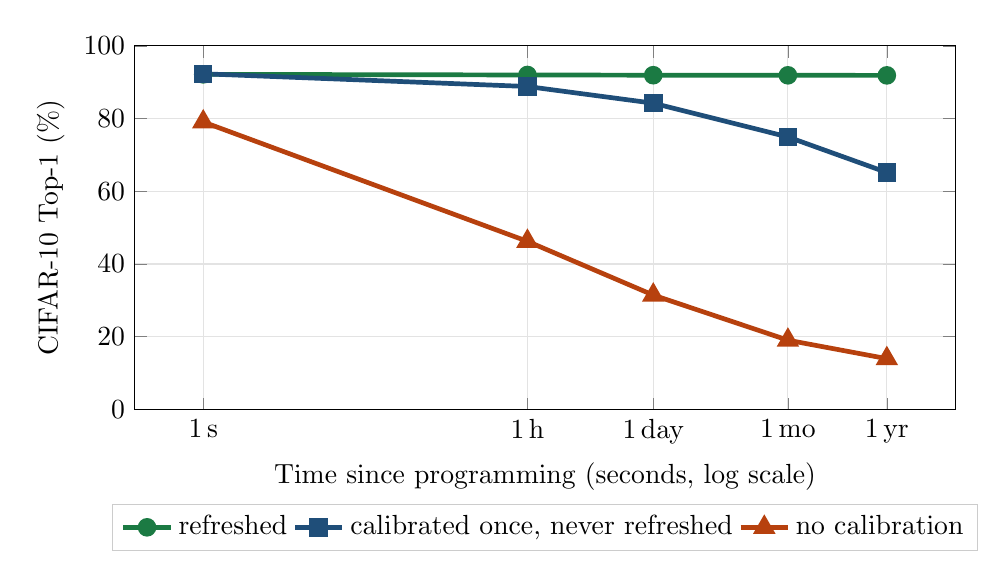
\begin{tikzpicture}
\begin{axis}[
  width=12cm,height=6.2cm,
  xlabel={Time since programming (seconds, log scale)},
  ylabel={CIFAR-10 Top-1 (\%)},
  xmode=log,ymin=0,ymax=100,grid=major,grid style={gray!22},
  xtick={1,3600,86400,2592000,31536000},
  xticklabels={1\,s,1\,h,1\,day,1\,mo,1\,yr},
  legend style={at={(0.5,-0.26)},anchor=north,legend columns=3,draw=gray!40},
]
\addplot[good,line width=1.7pt,mark=*,mark size=2.5pt]
  coordinates {(1,92.15)(3600,91.98)(86400,91.92)(2592000,91.89)(31536000,91.87)};
\addlegendentry{refreshed}
\addplot[acc,line width=1.7pt,mark=square*,mark size=2.5pt]
  coordinates {(1,92.31)(3600,88.81)(86400,84.22)(2592000,74.94)(31536000,65.17)};
\addlegendentry{calibrated once, never refreshed}
\addplot[warm,line width=1.7pt,mark=triangle*,mark size=3pt]
  coordinates {(1,79.06)(3600,46.23)(86400,31.45)(2592000,19.05)(31536000,13.97)};
\addlegendentry{no calibration}
\end{axis}
\end{tikzpicture}
\caption{Drift at $B=32$. A calibration computed once at manufacture decays
badly --- 27 points lost after a year. Recomputing it from the drifted array
holds accuracy flat indefinitely.}
\end{figure}

\begin{warnbox}{This forced an honest weakening of the claim}
We would like to say ``compile-time calibration''. Drift says we cannot. The
honest claim is \textbf{calibration with periodic refresh}.

The saving grace is that drift is a power law, so damage accumulates with the
\emph{logarithm} of time. Refreshing at 1 minute, 1 hour, 1 day, 1 week, 1
month and 1 year --- roughly \textbf{ten refreshes over the entire product
lifetime} --- bounds the error to well under a point. A refresh reads the
array and recomputes one constant per column. That is cheap and it folds into
the block-scale multiply already in the datapath.

We also got the refresh mechanism wrong at first. Recomputing only the loading
constant left 15.7\% residual error --- \emph{worse} than leaving it stale.
The reason: drift shrinks the weights themselves, and that scale error
dominates the loading error. The fix was to add a least-squares per-column
gain folded into the block scale, which corrects both at once.
\end{warnbox}


\section{How much do the drift assumptions matter?}

The drift conclusion rests on $\sigma_\nu$, the cell-to-cell spread in the
drift exponent, which is the least certain input in the entire model. Rather
than assert one value, it was swept.

\begin{table}[h]
\centering
\caption{Drift-exponent spread sweep, $B{=}128$, one year elapsed. ``Refresh
worth'' is the accuracy regained by recomputing the constants.}
\begin{tabular}{rrrr}
\toprule
$\sigma_\nu$ & stale & refreshed & refresh worth \\
\midrule
0.001 & 71.52 & 92.12 & $+20.60$ \\
0.002 & 71.53 & 92.03 & $+20.50$ \\
0.004 & 71.73 & 91.73 & $+20.00$ \\
0.008 & 73.36 & 90.54 & $+17.18$ \\
0.016 & 77.91 & 80.29 & $\mathbf{+2.38}$ \\
\bottomrule
\end{tabular}
\end{table}

\begin{keybox}{The boundary of the refresh claim}
Refresh holds within 2 points of the ceiling up to $\sigma_\nu = 0.004$ and
\textbf{begins failing at 0.008}. By 0.016 refreshing is nearly worthless.

The operating assumption of 0.004 sits right at the edge of the safe region.
The honest statement is therefore: \emph{``periodic refresh restores accuracy
to within one point provided the cell-to-cell drift-exponent spread stays
below roughly 0.008; beyond that, drift rather than the divider limits tile
height.''} Stating the boundary is far stronger than asserting the point.
\end{keybox}

\section{Confirming the mechanism rather than just observing it}

An earlier observation --- that stale-calibration loss falls as tile height
grows --- was made \emph{after} looking at the data, which is the weakest kind
of claim. The proposed explanation, that the error scales with
$\Rs \cdot \Gcol$, makes a falsifiable prediction: the tile-height trend must
strengthen as $\Rs$ grows and wash out as it shrinks.

\begin{table}[h]
\centering
\caption{Stale-calibration cost (points below the ceiling after one year with
no refresh) against sense resistance and tile height. Less negative is better.}
\begin{tabular}{rrrrrr}
\toprule
$R_s$ ($\Omega$) & $B{=}32$ & $B{=}64$ & $B{=}128$ & $B{=}256$ & spread \\
\midrule
5  & $-31.56$ & $-28.32$ & $-35.16$ & $-26.83$ & $-4.73$ \\
10 & $-29.47$ & $-25.44$ & $-29.43$ & $-20.57$ & $-8.90$ \\
20 & $-25.69$ & $-20.56$ & $-21.08$ & $-12.88$ & $-12.81$ \\
40 & $-19.66$ & $-13.67$ & $-12.18$ & $-6.38$ & $-13.28$ \\
80 & $-12.03$ & $-7.46$ & $-5.54$ & $-2.89$ & $-9.14$ \\
\bottomrule
\end{tabular}
\end{table}

Stale cost shrinks monotonically with $R_s$ at every tile height. The ordering
across tile heights is clean and monotonic at $R_s \geq 20\,\Omega$ but
scrambled at $R_s = 5\,\Omega$, exactly where the loading term is too small to
dominate.

\begin{saybox}{Why this matters more than the numbers}
``The trend was found by looking at data, so we treated it as a hypothesis
rather than a result. The mechanism predicts it should scale with $R_s$. We
swept $R_s$ over sixteen-fold and the prediction held. That converts an
observation into an explanation, and it answers the objection that the trend
was cherry-picked after the fact.''
\end{saybox}

%=====================================================================
\chapter{How Many ADC Bits Do We Need?}

The ADC dominates energy and area, and \jargon{SAR} ADC energy scales as
$2^N$ for $N$ bits. Every bit removed halves the cost; going from 8 bits to 6
divides the ADC energy by four. So this question is worth real money.

\begin{table}[h]
\centering
\caption{ADC resolution sweep, gain-calibrated, full test set. ``Exact'' means
an infinitely precise ADC.}
\begin{tabular}{crrrrrc}
\toprule
$B$ & 4 bits & 5 bits & 6 bits & 8 bits & Exact & Required \\
\midrule
32  & 74.88 & 91.27 & 92.41 & 92.47 & 92.42 & \textbf{6} \\
64  & 66.93 & 90.97 & 92.27 & 92.47 & 92.47 & \textbf{6} \\
128 & 77.18 & 91.43 & 92.43 & 92.70 & 92.81 & \textbf{6} \\
256 & 77.88 & 90.85 & 92.01 & 92.49 & 92.43 & \textbf{6} \\
\bottomrule
\end{tabular}
\end{table}

\begin{keybox}{The structural finding: the requirement is flat in $B$}
Six bits suffice at \emph{every} tile height. An eight-times taller tile needs
no extra ADC resolution.

This matters more than it looks. The worry with tall tiles is that they
produce a wider range of output values and therefore demand a finer ADC ---
which would hand back exactly the efficiency you gained by amortising the ADC
over more rows. \textbf{It does not happen.} The saving is real and it is
kept.
\end{keybox}

\begin{warnbox}{A second correction, same cause as the first}
An earlier draft claimed \emph{five} bits sufficed. That was measured at
1000--2000 images. On the full test set, five bits costs 1.15--1.58 points at
every $B$. The requirement is six.

Both retractions in this document have the same root cause: a number that
looked settled at small sample size. The rule adopted afterwards --- re-run
anything you intend to quote, on the full test set --- is worth stating as a
lesson learned.
\end{warnbox}


%=====================================================================
\chapter{What the Model Leaves Out}
\label{ch:wire}

The calibration corrects one thing exactly: the shared sense resistor. Real
interconnect has other parasitics, and honesty requires measuring them rather
than hoping they are small.

\section{Solving the whole mesh}

The closed-form model treats the wordline as an ideal voltage source and the
bitline as a single node. A separate solver drops both assumptions and solves
the full two-dimensional resistive mesh --- every wordline segment, every
bitline segment, every crosspoint --- as one sparse linear system.

Its self-test asserts that with ideal wires it reproduces the closed-form
model to $8.8\times10^{-8}$ relative. That agreement is what makes any
\emph{difference} at nonzero wire resistance trustworthy as physics rather
than a solver bug.

\begin{table}[h]
\centering
\caption{Each parasitic isolated, $M{=}128$. The sanity row must be near zero
after calibration; anything far above it is an effect the per-column constant
does not model.}
\begin{tabular}{lrr}
\toprule
Case & raw error & \textbf{after calibration} \\
\midrule
ideal wires (sanity check) & 71.3\% & \textbf{0.0002\%} \\
wordline metal 0.5\,$\Omega$ & 71.8\% & 1.82\% \\
wordline driver 50\,$\Omega$ & 78.3\% & \textbf{25.4\%} \\
bitline metal 0.5\,$\Omega$ & 84.8\% & \textbf{49.1\%} \\
bitline metal 1.0\,$\Omega$ & 89.1\% & 64.0\% \\
\bottomrule
\end{tabular}
\end{table}

\section{The uncomfortable finding}

Wordline \emph{metal} --- the parasitic everyone worries about --- is mild.
The two that hurt are \textbf{driver output resistance} and \textbf{bitline
metal resistance}.

The reason is structural. The correction $1 + \Rs\Gcol$ treats the bitline as
a single lumped node. Real bitline resistance is \emph{distributed}: a cell in
row 0 and a cell in row 127 see different accumulated IR on the way to the
sense node. No single per-column scalar can represent that.

\begin{warnbox}{Does a fitted constant rescue it? No.}
A per-column gain was fitted by least squares on one set of activation
patterns and tested on \emph{unseen} ones --- the only version of the test that
means anything, since a gain fitted and evaluated on the same data would look
perfect regardless.

\begin{center}
\begin{tabular}{rrrr}
\toprule
$M$ & raw & calibrated & + fitted gain (held out) \\
\midrule
32 & 57.7\% & 35.9\% & 14.1\% \\
64 & 70.1\% & 40.6\% & 17.7\% \\
128 & 87.8\% & 55.9\% & 47.4\% \\
256 & 91.6\% & 62.8\% & \textbf{68.7\%} \\
\bottomrule
\end{tabular}
\end{center}

At $M{=}32$ a fitted constant recovers most of it. At $M{=}256$ it makes
things \emph{worse} --- the fit does not transfer to unseen activations at all.
And even the best case, 14.1\%, is five orders of magnitude away from the
0.0002\% the sense-resistor calibration achieves.
\end{warnbox}

\section{What this does to the claim}

\begin{keybox}{The claim, narrowed to what the evidence supports}
\textbf{Before:} ``the analog error is a compile-time constant.''

\textbf{After:} ``the shared-sense-resistor loading term is exactly
correctable at compile time. Distributed wire parasitics are not, and are
reported separately.''

That is a smaller claim. It is still a real one --- the term being corrected is
the one that causes the accuracy collapse in the first place --- and it is a
claim that survives contact with a mesh solver, which the larger version does
not.
\end{keybox}

These runs use assumed wire resistances on random tiles, not the trained
network with a real metal pitch. The right next step is a PDK metal pitch,
which would say whether $R_{bl}$ is nearer 0.1 or 1.0\,$\Omega$ --- the
difference between a 17\% and a 64\% residual.

%=====================================================================
\chapter{Where ReRAM Actually Wins}

An honest evaluation has to say where the technology does \emph{not} help.
ReRAM's advantage is not raw compute throughput. It is memory.

\section{Density, standby power, and data movement}

\begin{table}[h]
\centering
\caption{ReRAM against 6T SRAM for the same 11.16 M weights at 65\,nm.}
\begin{tabular}{lrrl}
\toprule
Metric & ReRAM & SRAM & Advantage \\
\midrule
Weight array area (2-bit weights) & 3.77 mm² & 13.20 mm² & $3.5\times$ \\
vs.\ FP32 weights in SRAM & 3.77 mm² & 211.2 mm² & $56\times$ \\
Standby power & 0 mW & 2.68 mW & structural \\
Weight-fetch energy (reuse = 1) & 0 pJ/MAC & 0.100 pJ/MAC & structural \\
\bottomrule
\end{tabular}
\end{table}

Two of these are infinite rather than large, and the reason is structural
rather than a matter of degree. A non-volatile cell needs no power to
remember. A weight that is physically part of the computation needs never to
be fetched.

That last point deserves emphasis. In a conventional accelerator, moving a
weight from memory into the multiplier costs far more energy than the
multiplication itself. In a crossbar the weight \emph{is} the multiplier, so
that cost is not reduced --- it does not exist.

\section{The efficiency result}

\begin{table}[h]
\centering
\caption{Baseline versus proposed design. The baseline is not a straw man ---
it is what you get by building FP2 and a conventional passive-readout crossbar
exactly as each is specified.}
\begin{tabular}{lrr}
\toprule
 & Baseline & \textbf{Proposed} \\
\midrule
Block size / tile height $B = M$ & 32 & \textbf{128} \\
Per-column gain calibration & no & \textbf{yes} \\
ADC resolution & 8 bit & \textbf{6 bit} \\
\midrule
CIFAR-10 Top-1 & 77.66\% & \textbf{92.43\%} \\
Gap to FP2-digital ceiling & $-15.15$ pts & $\mathbf{-0.38}$ pts \\
Energy per MAC & 0.323 pJ & \textbf{0.0237 pJ} \\
Energy efficiency & 6.2 TOPS/W & \textbf{81.3 TOPS/W} \\
\bottomrule
\end{tabular}
\end{table}

\begin{keybox}{Why both improve at once}
Normally accuracy and efficiency trade against each other. Here they move
together, because a single change unlocks both.

Removing the loading error makes tall tiles \emph{usable}. Tall tiles amortise
the ADC over four times as many rows. And because the ADC requirement is flat
in $B$, the 8-bit converter can also drop to 6 bits, dividing its energy by
four again.

\textbf{$+14.77$ accuracy points and $13.1\times$ energy efficiency,
simultaneously.}
\end{keybox}

\section{Writing is brutally expensive}

Reprogramming a ReRAM cell costs roughly 100 pJ. Reading one costs about
0.001 pJ --- five orders of magnitude less.

The consequence is architectural. If the network does not fit on the chip all
at once, and you swap weights in and out, you pay that write cost constantly.
Our model puts the \textbf{break-even batch at about 2{,}200 images}: below
that, the chip spends more energy writing weights than computing with them
and is better described as a write engine than an accelerator.

\begin{warnbox}{This is a real limitation, and it should be stated plainly}
The design only makes sense \emph{fully weight-stationary} --- every weight
gets its own permanent cells. At $B=128$ our model reports 412\,mm² of die
area for ResNet-18 fully resident, which is not manufacturable at 65\,nm.

The honest framing: this is a \emph{scaled-node} argument. The area shrinks
with the square of feature size, so what is impossible at 65\,nm is
comfortable at 7\,nm. LLaMA-7B at FP2 needs ${\sim}2265$\,mm² at 65\,nm but
only ${\sim}26$\,mm² at 7\,nm.
\end{warnbox}

\section{Independent cross-check against NeuroSim}

NeuroSim V1.4 is a widely used, independently developed CIM simulator. Running
a comparable configuration:

\begin{table}[h]
\centering
\caption{Cross-check against NeuroSim V1.4.}
\begin{tabular}{lrr}
\toprule
 & This work & NeuroSim \\
\midrule
ADC share of energy & 55.6\% & 68.0\% \\
ADC share of area & 55.2\%$^\dagger$ & 19.2\% \\
Energy efficiency & 13.8 TOPS/W & 30.3 TOPS/W \\
\bottomrule
\end{tabular}
\end{table}

$^\dagger$\,\textbf{Different denominators, and the row is only honest with
this footnote.} Our 55.2\% is of \emph{tile} area --- array, converters, input
drive and accumulation. NeuroSim's 19.2\% is of \emph{chip} area, which also
contains interconnect, global buffer and pooling. The numbers are not in
conflict and must not be read as a disagreement.

Different tool, different methodology, same qualitative conclusion: the ADC
is a leading cost. NeuroSim's area figure comes from transistor-level sizing and is
better grounded than ours, so we adopt it.

\section{The chip area breakdown, and a lesson about searching}

For a long time this project believed that seventy per cent of NeuroSim's
reported chip area was unaccounted for --- that the printed components did not
add up to the printed total, and that an area argument therefore could not be
made. That belief was wrong, and how it survived is worth recording.

The components were being extracted from the log with a text search that
required the word ``area'' in the line. NeuroSim prints this:

\begin{quote}\small\ttfamily
Other Peripheries (e.g.\ decoders, mux, switchmatrix, buffers, IC, pooling and
activation units) on chip : 1.15e+07um\^{}2
\end{quote}

That line contains neither ``area'' nor ``array''. It was silently dropped,
and a dropped component looks exactly like missing silicon. Two other lines
were missed the same way. \textbf{A search that fails and a quantity that is
genuinely absent produce identical output, and only one of them is a finding.}

The fix was to match on the \emph{unit} instead --- any line of the form
\texttt{label : number um\^{}2} --- so the label can be anything. With that,
the breakdown closes.

\begin{table}[h]
\centering
\caption{NeuroSim V1.4 chip area, VGG-8, 65\,nm. Total $80.06$\,mm².}
\begin{tabular}{lrr}
\toprule
Component & Area (\textmu m²) & Share \\
\midrule
CIM array           & 21{,}031{,}200 & 26.3\% \\
Accumulation circuits & 16{,}177{,}500 & 20.2\% \\
ADC                 & 15{,}384{,}400 & 19.2\% \\
Interconnect        & 12{,}141{,}100 & 15.2\% \\
Other peripheries   & 11{,}549{,}600 & 14.4\% \\
\midrule
Named subtotal      & 76{,}283{,}800 & 95.3\% \\
Residual            &  3{,}772{,}300 &  4.7\% \\
\bottomrule
\end{tabular}
\end{table}

The $4.7\%$ residual is not mysterious either. Reading
\texttt{ChipCalculateArea} in \texttt{Chip.cpp}, nine statements add to the
area accumulator, and several of them --- the global H-tree or bus, the global
buffer, pooling, global accumulation, ReLU and sigmoid --- have no
corresponding print. Name it ``global buffer, interconnect and activation
units'' and move on.

\begin{keybox}{What this changes}
\textbf{The ADC is not the largest area term.} At 19.2\% it sits third, behind
the array at 26.3\% and accumulation at 20.2\%. Our own tile-level model puts
the ADC at 55\%, and both can be true: the tile-level figure excludes
interconnect, global buffer and pooling, so it is a percentage of a much
smaller denominator. \textbf{Always state which denominator is being used.}
Putting 55\% and 19.2\% in the same table without that qualification is the
kind of thing a reviewer catches.

An area \emph{improvement} can now be argued properly, because the breakdown
closes: run the baseline and proposed configurations and difference them
component by component, with \texttt{neurosim\_area\_breakdown.py --log A
--log B}. Attribute any saving to the component that moved. If the total falls
while the array stays fixed, the saving came from the converters, and that is
a different claim from a density claim.
\end{keybox}

\begin{warnbox}{Two caveats on this comparison}
\textbf{One.} NeuroSim runs VGG-8; we run ResNet-18. This is not like-for-like
and must be labelled as such.

\textbf{Two.} The device conversion is only half applied. NeuroSim's C++ core
carries our device parameters correctly, but its Python wrapper has a
\emph{separate} \texttt{--onoffratio} parameter that was still at its default
of 10 against our device's 403. The comparison must be re-run before it is
quoted in a paper.
\end{warnbox}

%=====================================================================
\chapter{Does It Transfer to Transformers?}
\label{ch:transformers}

CNNs are one workload. A reviewer will ask whether the result is specific to
them. So we tested a LLaMA-architecture language model.

\section{What can and cannot go on a crossbar}

\begin{table}[h]
\centering
\caption{Transformer layer mapping.}
\begin{tabular}{lll}
\toprule
Operation & Mappable? & Why \\
\midrule
q, k, v, o projections & \textbf{yes} & static weights \\
gate, up, down (FFN) & \textbf{yes} & static weights \\
$Q K^{\!\top}$ (attention scores) & no & activation $\times$ activation \\
$A V$ (weighted values) & no & activation $\times$ activation \\
\bottomrule
\end{tabular}
\end{table}

A crossbar stores something fixed. Attention multiplies two things that both
change every token, so there is nothing to program into a cell that stays put,
and reprogramming per token is hopeless at 100 pJ per cell. \textbf{The
attention core stays digital.} This is a genuine architectural limitation and
the paper must say so.

\section{The negative result, reported honestly}

Applying FP2 post-training quantization to LLaMA-160M destroys it: perplexity
goes from 28.02 to 445{,}867.

The diagnosis is clean. \textbf{69.5\% of weights round to zero.} LLM weight
distributions are far more heavy-tailed than a CNN's --- each block's scale is
set by a single outlier, and everything else in the block is then small enough
relative to that scale that it rounds away. A simple Gaussian calculation
predicts about 52\%; the real distribution gives 69.5\%.

\begin{keybox}{This is the quantizer's failure, not the crossbar's}
It is essential to keep these separate. The perplexity collapse is caused by
2-bit quantization of a heavy-tailed weight distribution without retraining.
It has nothing to do with the crossbar.

Conflating the two would be the first thing a reviewer catches.
\end{keybox}

\section{Isolating the crossbar claim}

Since perplexity cannot separate the two effects, we measured the thing our
contribution is actually about: \textbf{readout error}. We hooked all 84
target linear layers, captured the real activations the model produces, and
pushed them through the crossbar three ways --- ideal, raw, and calibrated.

\begin{table}[h]
\centering
\caption{Per-layer readout error on real LLaMA-160M activations, $B = 128$,
6-bit ADC, mean over 84 layers.}
\begin{tabular}{lrr}
\toprule
 & Raw & \textbf{Calibrated} \\
\midrule
Mean relative readout error & 27.7\% & $\mathbf{2.08\times10^{-5}}$\% \\
Signal-to-noise ratio & ${\sim}11$ dB & $\mathbf{{\sim}134}$ \textbf{dB} \\
\bottomrule
\end{tabular}
\end{table}

134 dB is float32 machine precision. The loading error is not reduced --- it
is \emph{gone}.

\begin{saybox}{How to say this}
``Six orders of magnitude, across 84 layers of a real transformer driven by
real activations. The heavy-tailed weight distribution that wrecks 2-bit
quantization has no effect at all on the calibration, and the reason is
structural: the correction depends only on column conductance sums, never on
how the weights are distributed. So the contribution transfers from CNNs to
transformers unchanged --- and we can show that even though the quantized
language model itself is unusable without retraining.''
\end{saybox}

%=====================================================================
\part{Defending the Work}
\chapter{What Is Genuinely New}

\section{The claimed contributions}

\begin{enumerate}[leftmargin=1.6em]
  \item \textbf{Per-column loading-gain calibration turns crossbar tile height
        from a binding constraint into a free parameter.} Exact rather than
        approximate, one constant per column, folded into a multiply that
        already exists, requiring no per-cell read-back.
  \item \textbf{Blind calibration survives realistic device variability} ---
        under one point at $\sigma = 20\%$, computed from nominal
        conductances. Write-verify buys nothing, which is a useful practical
        result.
  \item \textbf{$B = M$: block-floating-point block size and CIM tile height
        are one physical parameter.} We believe this is the first joint
        accuracy / SNR / energy characterisation of that coupling.
  \item \textbf{Methodological: additive-Gaussian analog error models cannot
        express a systematic gain}, so work built on them structurally cannot
        find this failure mode. This is the first circuit-exact end-to-end
        evaluation validated against exhaustive SPICE across every tile of
        every layer.
  \item \textbf{QAT makes block size a hardware-only parameter} --- with
        retraining, accuracy is flat in $B$, so the block size can be chosen
        purely for the circuit's benefit.
\end{enumerate}

\section{The most likely challenge, and the answer}

\begin{warnbox}{``Compensating crossbar loading is not new.''}
Correct, and you should concede it immediately rather than defend it.
IR-drop and loading compensation in crossbars is an established area.

The narrower claims that survive:
\begin{itemize}[leftmargin=1.3em]
  \item The correction is \emph{exact}, not a fitted approximation, and we
        show the algebra collapsing to the ideal product.
  \item It requires \emph{no read-back} --- blind, from nominal values, and we
        measure that this is sufficient under 20\% device spread.
  \item It is tied specifically to \emph{block floating point}, where it
        removes a constraint that the number format itself imposes. The
        $B = M$ framing is, as far as we know, new.
  \item The 2T2R ordering matters and is not obvious: correcting each bitline
        before subtraction is what makes it exact.
\end{itemize}

A literature search on ``IR drop compensation ReRAM crossbar'',
``conductance-dependent output scaling CIM'', and ``sneak-path calibration
in-memory computing'' should be completed before the introduction is written,
because it decides whether the paper says ``first to'' or ``unlike prior
work''.
\end{warnbox}


%=====================================================================
\chapter{Standing Against Prior Work}

Compensating crossbar non-idealities is a crowded field. This chapter names
the competing approaches and states honestly which parts of the contribution
survive contact with them.

\section{The landscape}

\begin{table}[h]
\centering
\caption{Existing approaches to crossbar non-ideality. The two in bold are
direct threats and must be addressed in the introduction, not left for a
reviewer to raise.}
\begin{tabular}{p{3.4cm}p{2.4cm}p{4.4cm}}
\toprule
Approach & Level & Cost \\
\midrule
Weight pre-distortion (non-ideality-aware training) & algorithmic & requires retraining \\
\textbf{BatchNorm recalibration} & software & retraining-free; needs validation data \\
\textbf{Op-amp virtual ground (TIA)} & circuit & one op-amp per column \\
Peripheral current injection & mixed-signal & op-amps, current mirrors \\
Sparsification & algorithmic & accuracy/sparsity trade \\
\bottomrule
\end{tabular}
\end{table}

\section{Threat one: why not just use a transimpedance amplifier?}

\begin{warnbox}{The most dangerous question in the viva}
A transimpedance amplifier holds the bitline at \emph{true} virtual ground.
With $v_{\mathrm{bl}} = 0$ the term $1 + \Rs\Gcol$ never arises at all.

So the error being corrected is a consequence of choosing passive resistive
sensing. Left unaddressed, the entire work reads as an elaborate solution to a
self-inflicted problem.
\end{warnbox}

The answer is not that the circuit fix is impossible --- it is that it is not
free, and the cost can be priced on the same tile.

\begin{table}[h]
\centering
\caption{What per-bitline transimpedance sensing would cost, $M{=}128$,
$K{=}16$. One amplifier per sensed bitline, and two converters per column are
already required by the calibration, so 32 amplifiers. Amplifier area and bias
are placeholders for a compact two-stage OTA at 65\,nm --- 1000\,µm² and 10\,µA
at 1.2\,V --- and are labelled \texttt{[ASSUM]} accordingly.}
\begin{tabular}{lrr}
\toprule
 & passive $+$ calibration & TIA sensing \\
\midrule
extra analog blocks & none & 32 op-amps/tile \\
tile area & 75\,369\,µm² & 107\,369\,µm² \\
 & & (\textbf{+42\%}) \\
die area, whole net & 411.8\,mm² & \textbf{586.6\,mm²} \\
added static power & 0 & 384\,µW/tile \\
 & & (\textbf{2.10\,W total}) \\
vs.\ measured array power & --- & $\mathbf{4.5\times}$ \\
correction cost & 1 multiply/col & none needed \\
\bottomrule
\end{tabular}
\end{table}

\begin{keybox}{The number that settles the argument}
The static power entry. \textbf{384\,µW per tile is 4.5$\times$ what the array
itself dissipates}, it is always on whether or not the chip is computing, and
across the network it adds \textbf{2.10\,W} to a design whose entire compute
budget is 274\,nJ per inference.

The digital correction costs one multiply per column, folded into a multiply
that already exists.
\end{keybox}

Three consequences, in order of how much they matter:

\begin{itemize}[leftmargin=1.4em]
  \item \textbf{Static power.} An op-amp burns bias current continuously. This
        is the entry that decides it.
  \item \textbf{Area.} 42\% more tile area, pushing an already-marginal
        411.8\,mm² die to 586.6\,mm².
  \item \textbf{Bandwidth.} The passive path settles in about 1\,ps against a
        12\,ns ADC conversion, so sensing is currently free in the latency
        budget. An amplifier would not be.
\end{itemize}

\begin{warnbox}{Be honest about what these numbers are}
The amplifier area and bias current are \texttt{[ASSUM]} placeholders, not PDK
values. The \emph{direction} of the conclusion is robust --- an amplifier per
column cannot be free, and static power cannot be zero --- but the exact
multiplier would move with a real op-amp design. Present it as an
order-of-magnitude argument, which is all it needs to be.
\end{warnbox}

\section{Threat two: BatchNorm recalibration}

BatchNorm recalibration is retraining-free, absorbs systematic column-current
attenuation, and is reported in the literature as landing within 0.16\% of
floating point. That is close to this work's claim by a much simpler route.

Four differences are real:

\begin{enumerate}[leftmargin=1.5em]
  \item \textbf{Exact, not fitted.} The correction here is an algebraic
        identity that collapses to the ideal product. BatchNorm recalibration
        is a statistical fit and leaves a residual.
  \item \textbf{Per-column, not per-layer.} BatchNorm parameters are per
        output channel and absorb a layer-average attenuation. The loading
        gain differs \emph{column to column} because $\Gcol$ differs, and that
        spread grows with tile height.
  \item \textbf{No data required.} BatchNorm recalibration needs a validation
        set; this correction is computed from the programmed conductances
        alone.
  \item \textbf{Works without BatchNorm.} The transformer layers measured in
        Chapter~11 have none, so a BatchNorm-based fix is simply unavailable
        there.
\end{enumerate}

\begin{table}[h]
\centering
\caption{BatchNorm recalibration measured against per-column calibration.
Full 10\,000-image test set, 6-bit ADC. BatchNorm statistics fitted on
train-split images.}
\begin{tabular}{rrrrrrr}
\toprule
$B{=}M$ & ideal & raw & BN & per-col & BN gap & per-col gap \\
\midrule
32  & 92.42 & 78.90 & 90.75 & \textbf{92.35} & $-1.67$ & $\mathbf{-0.07}$ \\
64  & 92.47 & 57.47 & 90.09 & \textbf{92.09} & $-2.38$ & $\mathbf{-0.38}$ \\
128 & 92.81 & 11.53 & 90.62 & \textbf{92.42} & $-2.19$ & $\mathbf{-0.39}$ \\
256 & 92.43 & 10.00 & 90.24 & \textbf{91.88} & $-2.19$ & $\mathbf{-0.55}$ \\
\bottomrule
\end{tabular}
\end{table}

\begin{warnbox}{A prediction that failed, and was dropped}
The argument above was that BatchNorm recalibration should degrade as tile
height grows, because a per-channel scalar cannot capture per-column variation
in $\Gcol$, and that variation widens with $M$.

\textbf{It was tested and it did not hold.} The BatchNorm gap averages
2.02 points below $B{=}128$ and 2.19 above it --- flat within noise. The
argument has been removed from the paper rather than quietly softened.
\end{warnbox}

\begin{keybox}{What the measurement gives instead, which is stronger}
\begin{itemize}[leftmargin=1.3em,itemsep=2pt]
  \item \textbf{Per-column wins at every tile height.} Worst gap 0.55 points
        against BatchNorm's 2.38, a factor of 4.3. At $B{=}32$ it is 0.07
        against 1.67, a factor of 24. A result that holds everywhere is
        cleaner than a trend that holds only at large $M$.
  \item \textbf{BatchNorm recalibration is a strong baseline, and saying so
        helps.} It lifts $B{=}256$ from chance (10.00\%) to 90.24\%. That a
        statistical fit absorbs most of the error is itself evidence the error
        is systematic rather than random.
  \item \textbf{Exactness, needing no calibration data, and working without
        BatchNorm all stand untouched.} Those were always the stronger three
        arguments.
\end{itemize}
\end{keybox}

\begin{saybox}{The detail to volunteer before it is asked}
``Our own gap grows slightly with tile height, from 0.07 to 0.55 points. That
is not calibration residual --- the correction is exact. It is 6-bit ADC
quantization, whose relative cost grows as the partial-sum range widens with
taller tiles. The ADC sweep shows the same effect independently.''
\end{saybox}

\begin{warnbox}{One discrepancy to report rather than hide}
Prior work reports BatchNorm recalibration landing within 0.16\% of floating
point. Here it lands 1.67--2.38 points short.

The likely reason is that their attenuation is IR-drop induced and roughly
uniform across a layer, whereas the shared-sense-resistor gain varies with
each column's programmed conductance --- so a per-channel affine has less to
grip on. The discrepancy should be stated, not resolved by quietly quoting
whichever number flatters.
\end{warnbox}

\section{What to claim, and what to concede}

\begin{keybox}{Concede immediately}
``First to compensate crossbar loading'' is \textbf{false}. IR-drop and
loading compensation is an established field. Conceding this in the first
paragraph costs nothing and buys credibility for the narrower claims that
\emph{are} defensible.
\end{keybox}

\begin{keybox}{The claim that leads}
The strongest contribution is not the calibration --- it is the
\textbf{format--device match} and the $B{=}M$ coupling it forces.

Multi-level ReRAM reliably holds about \emph{three} states. FP2's five signed
levels need only \emph{three magnitudes}, because 2T2R supplies the sign. So
FP2 lands exactly on what the device can physically hold: INT8 would need 256
levels or eight cells per weight; binary discards the dynamic range block
floating point exists to provide.

FP2 was designed for digital packing efficiency, with no reference to
resistive memory. That it coincides with the three-state limit of a ReRAM cell
is a genuine co-design observation --- and once FP2 is the format, $B{=}32$ is
fixed, and $B{=}M$ forces that onto the crossbar. Every later step then follows
from a physical constraint rather than a design preference.
\end{keybox}

\begin{saybox}{The whole argument in the order it should be told}
\begin{enumerate}[leftmargin=1.4em,itemsep=2pt]
  \item FP2 is what a three-state ReRAM cell can hold.
  \item So the format is fixed, and with it $B = 32$.
  \item $B = M$, so the crossbar tile height is fixed too.
  \item Which forces a tile too short to amortise the ADC.
  \item The loading gain is what makes taller tiles fail.
  \item And it is exactly correctable, for one multiply per column.
\end{enumerate}
\end{saybox}

%=====================================================================
\chapter{Anticipated Questions}

\begin{description}[leftmargin=0pt,style=unboxed,itemsep=9pt]

\item[\textcolor{acc}{Why is the error a gain rather than noise?}]
Because the derivation gives $I_{\text{actual}} = I_{\text{ideal}} / (1 + R_s
G_{\mathrm{col}})$, and the denominator contains only the sense resistance and
the programmed conductances. No activation term appears. Anything that does
not depend on the data is not noise.

\item[\textcolor{acc}{Why must block size equal tile height?}]
A column produces one current, and that current must be multiplied by one
scale factor. If the column spanned two blocks, two different scales would
have to be applied to a sum that physics already combined. The information
needed to separate them is gone.

\item[\textcolor{acc}{Why three resistance states?}]
Two reasons that happen to agree. ReRAM reliability degrades sharply beyond
three or four levels. And FP2's five signed levels need only three
\emph{magnitudes}, because 2T2R supplies the sign. INT8 would need 256 states,
or eight cells per weight.

\item[\textcolor{acc}{Why not just use a smaller sense resistor?}]
It reduces the error but does not remove it, and the measured voltage
$I R_s$ shrinks with it --- so you trade a gain error for a signal too small
to digitise. Calibration removes the error exactly without touching the
signal.

\item[\textcolor{acc}{How do you know your simulator is right?}]
87{,}168 tiles --- every tile of every layer --- through ngspice, 357 million
MAC reads, zero errors, worst disagreement $3.41\times 10^{-7}$ percent.

\item[\textcolor{acc}{Why do accuracy and efficiency improve together?}]
One change unlocks both. Removing the loading error makes tall tiles usable;
tall tiles amortise the ADC over more rows; and because the ADC bit
requirement is flat in $B$, the converter also drops from 8 bits to 6, whose
energy scales as $2^N$.

\item[\textcolor{acc}{What is the weakest part of the work?}]
Three things, in order. \emph{Drift} forces the claim down from
``compile-time'' to ``with periodic refresh''. \emph{Die area} at 65\,nm is
412\,mm² fully resident, so the argument depends on scaled nodes.
\emph{Wordline IR drop} is not yet modelled, and unlike bitline loading it is
activation-dependent, so it would not be a compile-time constant --- this is
the most likely thing to weaken the contribution.

\item[\textcolor{acc}{Why did the LLaMA perplexity fail?}]
Because 2-bit post-training quantization of a heavy-tailed weight distribution
rounds 69.5\% of weights to zero. That is the quantizer, not the crossbar. The
crossbar's own contribution is measured separately as readout error, where
calibration reduces 27.7\% to $2\times10^{-5}$\%.

\item[\textcolor{acc}{Why not use a transimpedance amplifier?}]
It would work, and it would remove the error entirely. It also costs an
op-amp per column in area and static power, and its bandwidth would bound the
read cycle where the passive path currently settles in 1\,ps against a 12\,ns
conversion. The argument is that loading need not be fixed in the circuit,
not that it cannot be.

\item[\textcolor{acc}{How is BatchNorm recalibration different from this?}]
It is a per-layer statistical fit needing validation data; this is a
per-column algebraic identity needing none. It is also unavailable on networks
without BatchNorm, such as the transformer layers measured here.

\item[\textcolor{acc}{Is 81.3 TOPS/W a chip-level number?}]
No, and it should never be quoted as one. It counts array, converters and
accumulation. Adding interconnect and buffers at NeuroSim's 20.8\% share puts
the chip-level figure near 64 TOPS/W.

\item[\textcolor{acc}{How sensitive is the result to the ADC assumption?}]
Very. The figure of merit alone swings the headline between 81.3 and
142.2 TOPS/W, which is why all three variants are reported rather than one.

\item[\textcolor{acc}{What would you do next?}]
Model wordline IR drop; complete the novelty search; run ImageNet; and apply
QAT to the language model so the transformer result can be stated as
perplexity rather than only as readout error.

\end{description}

%=====================================================================
\chapter{Honest Limitations and Remaining Work}

\section{What is not yet done}

\begin{table}[h]
\centering
\caption{Remaining work, ordered by whether it blocks submission.}
\begin{tabular}{llp{6.4cm}}
\toprule
Priority & Item & Note \\
\midrule
Blocking & Novelty search & Decides whether the introduction claims priority. \\
Blocking & Re-run Pareto at 6-bit & Efficiency figures were computed at 5 bits and rescaled by hand. \\
Blocking & Regenerate figures 1--7 & They still carry $n=2000$ numbers. \\
\midrule
Important & Error bars & Ten seeds exist; tables currently print means only. \\
Important & Sweep drift exponent spread & The refresh conclusion rests on $\sigma_\nu = 0.004$, the least certain input. \\
Important & Level-mapping error & See below. \\
Important & NeuroSim re-run & At the correct on/off ratio, and VGG-8 vs ResNet-18 must be labelled. \\
\midrule
Strengthening & Wordline IR drop & The most likely remaining threat. \\
Strengthening & ImageNet & Strongest single credibility upgrade. \\
Strengthening & Read noise & Averages over a dot product, so likely benign --- worth showing. \\
Strengthening & Temperature & Both drift and conductance are strongly temperature dependent. \\
\midrule
Deferred & RTL / synthesis flow & Blocked: the Verilog top level has no behavioural ADC model, which is why RTL error has read N/A throughout. \\
Deferred & Tapeout-grade area & Needs a real PDK; everything is currently an assumption. \\
\bottomrule
\end{tabular}
\end{table}

\section{The level-mapping error}
\label{sec:levelerr}

Recall that HRS is not infinite resistance. Working through the actual device
numbers, the three programmed states do not land exactly on $\{0, 0.5, 1\}$:
\[
\frac{R_{\mathrm{MID}}}{R_{\mathrm{LRS}}} = \frac{1099.8}{542.8} = 2.0262
\quad\text{(should be exactly 2)}
\]
and finite HRS leakage subtracts a further 0.25\% from every level. The net
effect is that level $0.5$ is physically $0.491$ --- a $1.79\%$ error.

This is \emph{separate} from the readout error this project fixes, and it is
currently absorbed into what we call the digital ceiling. It is also
straightforwardly fixable: either trim $R_{\mathrm{MID}}$ at programming time,
or fold the measured ratio into the block scale factor. It should be
quantified and then either fixed or reported.

\section{Lessons that generalise}

\begin{warnbox}{The pattern behind every mistake made}
Five errors were caught and corrected during this work:
\begin{itemize}[leftmargin=1.3em]
  \item ``Taller columns are more variability tolerant'' --- retracted; it was
        sampling noise at $n=1000$.
  \item ``Five ADC bits suffice'' --- wrong for the same reason; six are
        needed.
  \item The hardware model's fallback array power was $30\times$ too high,
        making every efficiency figure pessimistic.
  \item A figure caption was hardcoded and kept claiming ``5 bits'' after the
        answer had changed to 6.
  \item Refreshing only the loading constant made drift \emph{worse}, because
        weight shrinkage dominates.
\end{itemize}

Every one is either a number that looked settled at small sample size, or a
caption that stopped tracking its data. The rule that follows: \textbf{re-run
anything you intend to quote, on the full test set, and derive captions from
the data rather than typing them.}
\end{warnbox}

%=====================================================================
\chapter{Summary}

\begin{keybox}{The complete argument in nine steps}
\begin{enumerate}[leftmargin=1.4em,itemsep=3pt]
  \item A ReRAM cell stores a number as a conductance. Ohm's law
        $I = V\!\cdot\!G$ makes reading it a multiplication.
  \item A grid of cells performs a full matrix--vector product in one
        electrical settling time.
  \item Each column needs an ADC, which dominates energy and area, so taller
        tiles are the main efficiency lever.
  \item FP2 stores weights as five levels with a scale shared across 32
        weights. Three resistance states plus 2T2R differential encoding
        express all five.
  \item A column produces one current and can therefore carry only one scale
        factor, so block size and tile height are the same parameter:
        $B = M$. FP2 wants 32; the circuit wants 128+.
  \item Built naively, accuracy collapses from 92\% to 10\% --- pure chance.
  \item The cause is $I_{\text{actual}} = I_{\text{ideal}}/(1 + R_s
        G_{\mathrm{col}})$, which depends only on programmed conductances.
        It is a known gain, not noise, and Gaussian error models cannot
        represent it.
  \item Correcting each bitline by its own constant before the differential
        subtraction collapses algebraically to the exact ideal product.
        Accuracy returns fully at every tile height.
  \item Tile height becomes free, the ADC drops to 6 bits, and the result is
        $+14.77$ accuracy points and $13.1\times$ energy efficiency at once ---
        verified against exhaustive SPICE, surviving 20\% device variability,
        and requiring periodic refresh to survive drift.
\end{enumerate}
\end{keybox}

\vspace{1em}

\begin{saybox}{If you have sixty seconds}
``We store 2-bit floating-point neural network weights directly in ReRAM
cells, so multiplication happens by Ohm's law. The format shares a scale factor
across 32 weights, and because a crossbar column produces a single current
that can only carry one scale, the block size is forced to equal the tile
height. That is a problem, because the circuit wants tall tiles to amortise the
ADC. When we built it, accuracy fell to random guessing. We found the cause
was not noise but a deterministic gain --- the output is attenuated by one
plus the sense resistance times the column conductance, which depends only on
the weights we programmed. Dividing it back out, one constant per column,
recovers the accuracy exactly. That frees the tile height, which lets us go
four times taller and drop the ADC from eight bits to six, giving fourteen
accuracy points and thirteen-fold energy efficiency simultaneously. It is
verified against SPICE on every tile of every layer, it survives twenty percent
device variability, and it transfers to transformers --- though it needs
periodic recalibration to survive conductance drift.''
\end{saybox}

\end{document}
